\setchapterpreamble[ur][.6\textwidth]{%
\dictum[Jean-Paul Sartre, \textit{La naus\'ee}]{%
Quand on veut comprendre une chose, on se place en face d'elle, tout seul, sans secours; tout le pass\'e du monde ne pourrait servir de rien. Et puis elle dispara\^{i}t et ce qu'on a compris dispara\^{i}t avec elle.}\vskip1em
}

\chapter[Successful by chance?]{Successful by chance? The power of mixed models and neutral simulations for the detection of individual fixed heterogeneity in fitness components}

\textbf{Timoth\'{e}e Bonnet*} and Erik Postma (2016) The American Naturalist 187(1):60-74\\

\section{Abstract}
Heterogeneity in fitness components consists of fixed heterogeneity due to latent differences fixed throughout life (e.g. genetic variation), and dynamic heterogeneity generated by stochastic variation. Their relative magnitude is crucial for evolutionary processes, as only the former may allow for adaptation. 
However, the importance of fixed heterogeneity in small populations has recently been questioned. Using neutral simulations (\NSM), several studies failed to detect fixed heterogeneity, thus challenging previous results from mixed models (\MM).
To understand the causes of this discrepancy, we estimate the statistical power and false positive rate of both methods, and apply them to empirical data from a wild rodent population.
    While \MM show high false positive rates if confounding factors are not accounted for, they have high statistical power to detect real fixed heterogeneity. In contrast, \NSM are also subject to high false positive rates, but always have low power. Indeed, \MM analyses of the rodent population data show significant fixed heterogeneity in reproductive success, whereas \NSM analyses do not.
   We suggest that fixed heterogeneity may be more common than is suggested by \NSM, and that \NSM are useful only if more powerful methods are not applicable and if they are complemented by a power analysis.

\textbf{Keywords: } \textit{Chionomys nivalis}; individual-based model; generalized linear mixed model; simulations; snow vole; statistical power\\
\textbf{Online enhancements: }
Online appendices. Data available from the Dryad Digital Repository: \url{http://dx.doi.org/10.5061/dryad.3cb61}.

\section{Introduction}

Within species, individual variation in lifetime reproductive success (LRS) is plentiful, with most individuals producing few or no offspring and a few individuals producing a large share of the next generation \parencite{Clutton1988,Stearns1992}. Given their skewed and heterogeneous nature, LRS distributions are unlikely to be solely shaped by unstructured environmental stochasticity. Instead, individuals seem to differ in their probability of surviving or reproducing \parencite{Kendall2011}.

Often, this individual heterogeneity in LRS is assumed to originate from latent individual differences which are fixed throughout an individual's life, i.e. that there is individual heterogeneity in frailty, quality or fitness \parencite[e.g.][]{Vaupel1979,Morris1998, Cam2000}. This is commonly referred to as fixed heterogeneity. Genetic variation is one source of fixed heterogeneity \parencite[e.g.][]{Keller2002,Ellegren2008}, but epigenetic, maternal and permanent environmental effects may also be important \parencite{Wolf2009,Turner2009}. This fixed variation is usually measured retrospectively; in some cases it may have arisen at fertilization, but it may also be shaped by the environment an individual experiences throughout its life, for instance through variation in habitat choice or through gene by environment interactions. It is important to distinguish fixed heterogeneity as it is used here\textemdash that is, the repeatability of individual performance\textemdash from other sources of variation that are not due to the properties of individuals (e.g. climatic variations among years). Indeed, only fixed differences among individuals can be the target of selection and allow for adaptation, provided that these fixed differences are passed on to the next generation\textemdash be it through genes \parencite{Keller2002}, philopatry \parencite{Schauber2011} or other processes \parencite{Bonduriansky2012}. 

Recent publications \parencite{Tuljapurkar2009,Steiner2010,Orzack2011,Steiner2012} have argued forcefully that invoking fixed differences among individuals (i.e. fixed heterogeneity) in fitness components is rarely required to explain the observed heterogeneity in LRS. Instead, they emphasize that due to the stochasticity of individual life histories, individual heterogeneity is expected even in populations of identical individuals \parencite{Caswell2011}. Indeed, if individuals take a random trajectory through the various life-history stages, and if these stages are associated with differential reproductive and survival rates, the population-level distribution of LRS may be skewed and heterogeneous. This type of heterogeneity is referred to as dynamic heterogeneity \parencite{Tuljapurkar2009}. Crucially, dynamic heterogeneity originates from differences among life stages, whereas fixed heterogeneity originates from variation in the properties of individuals.

Given that most life-history traits are heritable to some degree \parencite{Mousseau1987, Postma2014}, it is beyond doubt that some fixed heterogeneity is present in most wild populations. At the same time, the cumulative effects of individual histories on their realized lifespan and reproductive success are also unquestionable \parencite{Caswell2011}. What is subject to discussion, however, is the relative importance of fixed, versus dynamic, heterogeneity in shaping variation in LRS. \cite{Steiner2012} suggested that, at least in small populations, the drift generated by large life-history stochasticity is too large for fixed heterogeneity to play a significant role in shaping evolution and demography at the level of a single population. Instead, they have proposed dynamic heterogeneity as the null model to explain any observed heterogeneity. Only if this null model can be rejected should we consider an additional role for fixed heterogeneity in shaping variation in LRS or fitness components. 

\cite{Tuljapurkar2009} have suggested that an appropriate tool to test for fixed heterogeneity is provided by neutral simulations (\NSM hereafter), which generate summary statistics describing the distribution of LRS and the pattern of life-stage transitions expected in the absence of fixed heterogeneity. These expectations can subsequently be compared to their observed counterparts to detect departures from neutrality due to the existence of fixed heterogeneity. 

The application of \NSM to data for two sea bird populations \parencite{Steiner2010,Orzack2011}, as well as to a compilation of 22 vertebrate populations \parencite{Tuljapurkar2009} has been unable to reject the null hypothesis of neutrality, leading to the conclusion that dynamic heterogeneity alone can explain the observed variation in life histories in most populations. Indeed, we are aware of only one study in which \NSM rejected neutrality, for one of three reproductive parameters in a roe deer population \parencite{Plard2012}. 

In contrast to studies relying on \NSM, studies employing linear mixed models (hereafter \MM) commonly report evidence for fixed heterogeneity \parencite[e.g.][] {Cam2000,Royle2008,Chambert2013,Guillemain2013,Chambert2014}. Interestingly, \cite{Cam2013} have provided evidence for fixed heterogeneity in a data set for which the existence of fixed heterogeneity had been dismissed based on \NSM \parencite{Steiner2010}. However, \MM and \NSM differ in how they deal with data: \MM rely on repeated measurements of individuals, while \NSM use summary statistics aggregated at the population level. Compared to \MM, \NSM are thus less data-demanding, but might be less sensitive to statistical signals at the individual level. On the other hand, aggregation might allow \NSM to detect effects that emerge only at the population level and are invisible to \MM.
More formally, the discrepancy between \NSM and \MM suggests that they differ in either their type I (i.e. false positive) error rate, or in their type II error rate (i.e. power). For instance, the opposite conclusions reached by \NSM in \cite{Steiner2010} and \MM in \cite{Cam2013} may be the result of the statistical power of the \NSM being too low, preventing the detection of fixed heterogeneity (i.e. a type II error). Alternatively, \MM may have high rates of type I error, if the individual-level variances estimated by the \MM are spurious, or they are unduly interpreted as the mark of fixed heterogeneity.

Applying both methods to data with known properties allows for the estimation of both types of error rates and thereby provides insight into the ability of both methods to detect fixed heterogeneity. Unfortunately however, fixed heterogeneity is the result of latent, unobservable traits, which cannot be inferred without a modeling step \parencite{Cam2013}, and it is precisely the performance of this modeling step that we investigate here. Computer simulations provide a way around this problem, as they allow one to apply methods to data sets with known underlying properties \parencite[e.g.][]{DeVillemereuil2013,Brooks2013}.

Here, we simulate a series of longitudinal, individual-based, data sets through an algorithm that introduces varying amounts of fixed and dynamic heterogeneity in survival and reproduction. For illustrative purposes, these simulations are parametrized to match a population of snow voles (\textit{Chionomys nivalis}, Martins 1842) located in the Swiss Alps. In order to assess the type I and type II error rates of both \NSM and \MM, we subsequently analyze the simulated data sets using both methods. In a final step, we use these results to interpret the results of the application of both methods to the real snow vole data set. Figure \ref{figure:flow} shows a diagram summarizing our approach. Altogether, our results highlight the lack of statistical power of \NSM, but at the same time emphasize that \MM output should be interpreted with care. We discuss the origin of the discrepancy between \NSM and \MM, and what this tells us about the nature of biological variability.

\section{Material and methods}

\subsection{Data simulation}

The simulation model matches the life cycle of the population of snow voles which we use in the empirical comparison of both methods. The monitoring of this population is discussed in some detail in Appendix \ref{ap:snv}. Only two age classes are modeled (non-reproducing juveniles and reproducing adults), and there are no sex-specific or spatio-temporal effects on fitness components, as the uncertainty with respect to the appropriate specification of these models would introduce an additional layer of complexity \parencite[see e.g.][]{Cam2013}.
All simulated populations are monitored for 10 years. For every individual, we have perfect knowledge of survival and reproduction during the study period, but their fate beyond this period is unknown. Every year, a new cohort of 100 juveniles appears. After one year, these juveniles become adults and start reproducing. Every year, adults can reproduce once; the number of offspring produced by an individual is labeled annual reproductive success (ARS). In the real snow vole population, there is no apparent senescence in survival and the maximum age observed is four years old. Accordingly, in the simulations, adult survival probability does not vary with age until the fourth year, but all individuals still alive at that point die during the next winter. Mortality events occur after birth for juveniles and after reproduction for adults. A single sex is simulated, as the two sexes are generally analyzed separately in \NSM, and in \MM sex differences in the mean are accounted for by fitting sex as a fixed factor.

We define a scenario as a collection of simulation parameters. For each scenario, 1000 data sets were simulated, that is 1000 putative populations with the same underlying properties. In an attempt to detect evidence for fixed heterogeneity, each data set was then analyzed using \MM and \NSM. Note the potential for confusion between the simulation of the data sets on the one hand, and the neutral simulation method on the other. The latter is always referred to as \NSM. Simulations were carried out using a C++ program (available at \verb+https://github.com/timotheenivalis/FixDynHet+), using the pseudo-random number generator \verb+Mersenne Twister+ \parencite{Matsumoto1998} and a command file procedure following that of \verb+IBDsim+ \parencite{Leblois2009}. The analyses of the simulation output were all conducted in \verb+R 3.1.0+ \parencite{R2014}, using the package \verb+lme4+ (version 1.1-7) \parencite{Bates2014a}.

Due to demographic stochasticity \parencite[sensu][]{Fox2002}, all simulated data sets contain a baseline level of dynamic heterogeneity. Indeed, according to \cite{Tuljapurkar2009}, the presence of dynamic heterogeneity results in the ``scaled sequence entropy of the transition matrix between reproductive stages'' (hereafter simply referred to as entropy), being greater than zero, which is always the case here. Entropy measures the rate at which the diversity of life-history trajectories increases with their length, which is due to random transitions between stages with different survival probabilities and reproductive outcomes \parencite{Tuljapurkar2009}.

Beyond this baseline level of dynamic heterogeneity, heterogeneity in fitness components is introduced either as explicit fixed heterogeneity, or through a Markovian process. For the simulation of fixed heterogeneity, at birth, each individual receives a fixed quality as reproducer and survivor. These fixed qualities do not change over the course of its life. Therefore, some individuals intrinsically have a high probability to perform well, and some individuals have a high probability to perform poorly, irrespective of their past performance, as in a classic frailty model \parencite{Vaupel1979}. In contrast, for the simulations using a Markovian process, an individual's probability to survive and to achieve a certain ARS is not fixed, but changes at each time step and depends solely on its ARS the time step before. Therefore, these data contain dynamic heterogeneity only. However, some of this mimics fixed heterogeneity because individual performances can persist over time. Generalized linear mixed models were used to check that the properties of the simulated data sets matched the model and the parameters used to generate them (see Appendix \ref{ap:chpro}).

\paragraph{Simulations with explicit fixed heterogeneity}
At birth, every individual receives a quality as reproducer $q_{\rho,i}$, which is normally distributed with a mean of 0 and a variance equal to $\sigma_{\rho}^2$, i.e. \mbox{$q_{\rho,i}\sim$ {\fontfamily{pzc}\selectfont N }$(0,\sigma_{\rho}^2)$.} Individuals also receive a quality as survivor $q_{\phi,i}$, with \mbox{$q_{\phi,i}\sim$ {\fontfamily{pzc}\selectfont N }$(0,\sigma_{\phi}^2)$.} These qualities are fixed for the lifetime of an individual. Because trade-offs between survival and reproduction are not considered here, the two qualities are drawn independently for each individual. The variances $\sigma_{\rho}^2$ and $\sigma_{\phi}^2$ represent the amount of fixed heterogeneity in reproduction and survival, respectively. 

If individual $i$ is an adult at time $t$, its annual reproductive success, $\rho_{i,t}$, is drawn from a Poisson distribution,

\begin{equation}
\rho_{i,t} \sim \text{{\fontfamily{pzc}\selectfont P }}(\exp(\log(\mu_{\rho})+q_{\rho,i}))\text{,}
\end{equation}
where $\mu_{\rho}$ is the mean annual reproductive success. For an individual with $q_{\rho,i}=0$, i.e. the average individual in a population with fixed heterogeneity, the parameter of the Poisson distribution ($\exp(\mathrm{log}(\mu_{\rho})+q_{\rho,i})$) reduces to the population mean ARS ($\mu_{\rho}$). The qualities for reproduction ($q_{\rho,.}$) are normally distributed on the log-transformed scale of ARS.

The survival outcome of an individual $i$ at time $t$, $\phi_{i,t}$, is zero (death) if the individual is four years old, and otherwise is drawn from a Bernoulli distribution:

\begin{equation}
\phi_{i,t} \sim \text{{\fontfamily{pzc}\selectfont B }}( \mathrm{logit}^{-1}(\mathrm{logit}(\mu_{\phi}+j_{i,t}\beta_{j})+q_{\phi,i})) \text{,}
\end{equation} 
where $\mathrm{logit}(p)= \mathrm{log}(\frac{p}{1-p})$ and its inverse function $\mathrm{logit}^{-1}(x)=\frac{1}{1+\exp(-x)}$, where $j_{i,t}$ is a Boolean variable equal to 0 for adults and 1 for juveniles, and where $\beta_{j}$ is the difference between the mean survival probability of juveniles and adults. For an individual with $q_{\phi,i}=0$, the probability of survival ($\mathrm{logit}^{-1}(\mathrm{logit}(\mu_{\phi}+j_{i,t}\beta_{j})+q_{\phi,i})$) reduces to ($\mu_{\phi}+j_{i,t}\beta_{j}$), the age-specific mean survival probability. The qualities for survival ($q_{\phi,.}$) are normally distributed on the logit-transformed scale.

The mean of a log (or a logit) distribution is in general not equal to the log (or the logit) of the mean of this distribution (i.e. $\overline{\log(x)} \neq \log(\bar{x})$). Hence, Gaussian variance in individual qualities introduces a bias on the log or logit scale in the mean realized ARS and survival. If not corrected for, this bias causes the distributions of ARS and survival to deviate from their neutral expectations, which could be interpreted as evidence for fixed heterogeneity. To this end, the median individual qualities, $\tilde{q_{\rho}}$ and $\tilde{q_{\phi}}$, were iteratively modified so that the realized population means do not depend on the variances in individual qualities.

Because they are fixed for life, the individual qualities are the target of selection. Indeed, selection, i.e. the individual-level covariance between quality and relative LRS, increases with increasing variances ($\sigma_{\rho}^2$ and $\sigma_{\phi}^2$) (Appendix \ref{ap:sel}). It could thus be argued that in response to this selection, mean latent qualities should increase and their variances decrease over time. However, here we chose not to simulate a trans-generational response to selection, as this introduces an unnecessary layer of complexity: First, a phenotypic response to selection on components of fitness is not necessarily expected. For example, environmental deterioration, which may be the result of an increase in mean competitiveness \parencite{Fisher1958,Hadfield2011}, may mask a genetic change. Second, only the additive genetic part of the variation can respond to selection, and genetic variation may be renewed through migration, mutations and balancing selection \parencite{Fisher1958,Charlesworth2014}.
Therefore, simulating a response to selection would require much more complicated simulations and many more assumptions (e.g. an explicit genetic architecture for fitness, mechanisms to maintain genetic variation, competitive interactions). 
Finally, both \MM and \NSM are blind to temporal variation, as they compute statistics averaged over the whole data set, and even if a response to selection were apparent, it would have little effect on their performance.

The simulation framework outlined above closely matches the structure of the \MM later used to analyze the simulated data. Although we believe this simulation framework to be closest to biological reality, it could be argued that this may result in an overestimation of the ability of \MM to deal with real data. Therefore, two alternative simulation structures not exactly matching the structure of \MM were used. In the first, fixed heterogeneity was introduced on the original, rather than transformed, scale of survival probability and expected reproductive success. The results from this first alternative simulation structure did not differ qualitatively from the results obtained with the standard simulation structure, so they are presented in Appendix \ref{app:orsc}. The second alternative structure considers identical individuals, that is there is no explicit fixed heterogeneity, and a Markovian process with structured transition probabilities between reproductive stages and survival probabilities (see below).

\paragraph{Simulations with a Markovian process}
Simulations were carried out as previously described, except that ARS and survival probabilities depended on their previous state and not on fixed individual qualities. This matches the structure of the \NSM as proposed by \cite{Tuljapurkar2009} and is referred to as the ``full dynamic model'' in \cite{Plard2012}. Note that in this model, as shown in \cite{Plard2012}, the non-random transition probabilities of the Markovian process can be interpreted either as the result of fixed heterogeneity (if successful animals have a higher than average probability of remaining successful because of their individual properties, such as genetic quality) or of dynamic heterogeneity (if the persistence of success comes from the properties of reproductive stages rather than individuals, e.g. only individuals that have a territory can reproduce and these individuals are more likely than non-reproducers to have a territory next year). Indeed, for short lived species, a Markovian process produces among-individual variance because there are only a few observations per individual, and the first outcome of a Markov chain can have a big influence on the mean individual outcome. In long-lived species, on the other hand, mean individual performances will asymptotically approach the population mean. 

In these simulations, the ARS of individual $i$ at time $t$, $\rho_{i,t}$, follows:
\begin{align*}
&\rho_{i,t} \sim \text{{\fontfamily{pzc}\selectfont P }}(\mu_{\rho}) \text{; for second year individuals,}\\ 
&\rho_{i,t} \sim \text{{\fontfamily{pzc}\selectfont P }}(\mu_{\rho}+m(\rho_{i,t-1}-\mu_{\rho}))\text{; for older individuals,}
\end{align*}
where $\rho_{i,t-1}$ is the ARS of the focal individual the year before, $\mu_{\rho}$ is the mean ARS of the population and $m$ controls the strength of the  Markovian process, i.e. the degree to which current reproductive success depends on the previous reproductive success. Only positive values of $m$ were used in order to produce an individual persistence of ARS, which may mimic latent fitness (see below).\\
Similarly, the survival outcome of individual $i$ at time $t$, $\phi_{i,t}$, follows:
\begin{align*}
&\phi_{i,t} \sim \text{{\fontfamily{pzc}\selectfont B }}(\mu_{\phi}+\beta_{j}) \text{; for juveniles}\\
&\phi_{i,t} \sim \text{{\fontfamily{pzc}\selectfont B }}(\mathrm{logit}^{-1}(\mathrm{logit}(\mu_{\phi})+c(\rho_{i,t-1}-\mu_{\rho}) ))\text{; for adults,}
\end{align*}
where $\mu_{\phi}$ is the mean adult survival, $\beta_{j}$ is the difference between the mean survival of juveniles and adults, and $c$ controls the correlation between reproduction and survival. Survival probability at time $t$ depends on ARS at time $t-1$ rather than on previous survival, as the latter is always 1 for surviving individuals. Again, only positive values of $c$ were used to simulate persistence of the individual propensity to survive. The positive correlation between successive survival probabilities arises indirectly through the positive correlation between successive ARS, combined with the positive correlation between ARS and survival.

In the presence of allocation trade-offs between different life-history traits, or between successive expressions of the same life-history trait, negative correlations (i.e. $m < 0$) and autocorrelations (i.e. $c < 0$) could be expected. However, phenotypic correlations between life-history traits are often positive \parencite[][chapter 4]{Stearns1992}. This discrepancy is the result of the variance in resource acquisition, which is related to variance in latent fitness, being larger than the variance in resource allocation \parencite{vanNoordwijk1986}. Based on this, positive values of $c$ and $m$ are in line with the presence of variation in latent fitness. Indeed, a positive correlation between survival and reproduction is observed in the snow vole data (correlation between observed variation in survival and reproduction: Pearson's correlation, 0.097, 95\%CI $[-0.007;0.198]$. For the correlation between the latent propensities to survive and to reproduce, see Appendix \ref{ap:cor}

\paragraph{Simulation parameters}
The simulated mean survival probability from  year $t$ to year $t+1$ was 0.4 for juveniles and 0.2 for adults (observed means in snow voles: 0.403 and 0.219, respectively). ARS, averaged over adults, was set to 3, 10 or 50 offspring. For the real snow vole population, mean ARS values of 3 (resulting in a decreasing population size) and 10 (i.e. increasing population size) are within the range observed among years (noting that we include offspring of both sexes in ARS, while we analyze vital rates for only one sex), while the value 50 aimed at confirming the direction of the trend in test performance with respect to mean ARS. The variance in individual quality, either on the original scale or on a transformed scale, $\sigma_{\phi}^2$ and $\sigma_{\rho}^2$, took the values 0, 0.1, 0.5, 1 or 2. In simulations without fixed heterogeneity, the $m$ parameters took the values 0, 0.1, 0.2, 0.3, 0.4, 0.5, 0.6, 0.7, 0.8, 0.9 or 1, while the $c$ parameters took the values 0, 0.5 or 1. We had no a priori expectations for the heterogeneity parameters ($\sigma_{\phi}^2$, $\sigma_{\rho}^2$, $m$ and $c$) in the real snow vole population and thus selected the non-null values in a range from small to large relative to the mean survival and ARS.


%%%%%%%%%%%%%%%%%%%%%%%%%%%%%%%%%%%%%%%%%%%%%%%%%%%%%%%%%%%%%%%%%%%%%%%%%%%%%%%%%%%%%%%%%%%%%%%%%%%%
\subsection{Testing for fixed individual heterogeneity}
\paragraph{Neutral Simulations (\NSM)}
\NSM were carried out following \cite{Tuljapurkar2009}, but we used the ``full stochastic model'' proposed by \cite{Plard2012}. Compared to the original formulation of \NSM, the ``full stochastic model'' better isolates dynamic heterogeneity by making future states independent of the current state. Thereby it removes the non-stochastic component of transition probabilities and allows testing whether ``a given lifetime reproductive metric distribution is generated only by dynamic heterogeneity'' \parencite{Plard2012}. 

Briefly, individual life histories, starting as juveniles, are simulated by producing a sequence of ARS values, with the probability of each value of ARS corresponding to its frequency in the focal data set. Mortality events, with an age-specific probability estimated from the data set, are mapped to these individual trajectories. Subsequently, properties of the resulting LRS distribution, as well as of the transition matrix between life stages, are compared between the focal data set and that obtained using \NSM.

Here it is crucial to highlight some differences between the \NSM and the way in which we simulated the data sets to which they are applied. First and foremost, in \NSM the propensity to reproduce and to survive is identical for all individuals and never depends on the previous reproductive success. Second, in our simulations, ARS follows a Poisson distribution\textemdash all positive integers are possible values\textemdash whereas in \NSM, ARS are drawn from the ARS values observed in the focal data set, which can follow any distribution, and for instance may have gaps, multiple modes or extreme skewness. Third, in our simulations, mean survival probability is always 0.4 for juveniles and 0.2 for adults, while in \NSM these age-specific probabilities are the age-specific frequencies of survival that are realized in the focal data set. To sum up, our simulations are parametric and follow well defined distributions, while \NSM use empirical distributions and thereby stick to the data.

To test for a deviation from the neutral expectation, LRS distributions were compared using both Kolmogorov-Smirnov tests \parencite[used in][]{Steiner2010} and $\chi^2$ tests \parencite[used in][]{Plard2012}. Additionally, we calculated mean LRS, the variance in LRS, as well as the persistence of the reproductive stage transition matrix and its entropy following \cite{Plard2012}. Observed values greater than the 95\% quantile\textemdash or smaller than the 5\% quantile in the case of entropy, because more fixed heterogeneity should decrease entropy \parencite{Tuljapurkar2009}\textemdash of the neutral distribution were considered significantly different. 
The proportion of data sets for which a test is significant in the absence of simulated fixed heterogeneity gives the type I error rate, whereas the proportion of data sets for which a given test is not significant in the presence of simulated fixed heterogeneity gives the type II error rate. The \NSM method is computationally intensive, so to minimize computational time, we used the minimal number of \NSM per simulated data set beyond which statistical power did not change (Appendix \ref{ap:opnum}).

\paragraph{Mixed Models (\MM)}
Generalized linear mixed models (GLMMs) were used to estimate the variance in reproduction and survival attributable to fixed individual heterogeneity, as well as to test for its statistical significance. Significance of the variance components was assessed using Likelihood Ratio Tests (LRT) \parencite[see e.g.][]{Pinheiro2000,Crainiceanu2004}, assuming that the statistic follows an even mixture of $\chi_{1}^2$ and $\chi_{0}^2$ \parencite{Self1987}.
For survival, first a logistic model not allowing for individual-level heterogeneity was fitted:

\begin{equation}\label{firstsurv}
\mathrm{logit}(\phi_{i,t}) = \mu_{\phi}+\mathrm{Age}_{i,t}\text{ ,}
\end{equation}

where $\mu_{\phi}$ denotes the intercept and $\mathrm{Age}_{i,t}$ denotes the effect of age (juvenile or adult) of individual $i$ at time $t$.
In order to model individual-level heterogeneity, this model was subsequently expanded with an individual random intercept:

\begin{equation}\label{secondsurv}
\mathrm{logit}(\phi_{i,t}) = \mu_{\phi}+\mathrm{Age}_{i,t}+z_{\phi,i}\text{ ; with } z_{\phi}\sim \text{\fontfamily{pzc}\selectfont N }(0,\hat{\sigma_{\phi}}^2) \text{ .}
\end{equation}

Model \eqref{secondsurv} estimated the individual-level heterogeneity in survival probability, $\hat{\sigma_{\phi}}^2$. Moreover, a LRT comparing model \eqref{secondsurv} to model \eqref{firstsurv} tested for the significance of $\hat{\sigma_{\phi}}^2$.

Similarly, for ARS a first Poisson model without individual-level heterogeneity was fitted:
\begin{equation}\label{firstrepro}
\mathrm{log}(\rho_{i,t}) = \mu_{\rho}+ \mathrm{Age}_{i,t} \text{ ,}
\end{equation}
where $\mu_{\rho}$ denotes the intercept and $\mathrm{Age}_{i,t}$ denotes the effect of age. Subsequently, an individual random intercept was included to model individual-level heterogeneity:

\begin{equation}\label{secondrepro}
\mathrm{log}(\rho_{i,t}) = \mu_{\rho}+\mathrm{Age}_{i,t}+z_{\rho,i}\text{ ; with } z_{\rho}\sim \text{\fontfamily{pzc}\selectfont N }(0,\hat{\sigma_{\rho}}^2) \text{ .}
\end{equation}

Model \eqref{secondrepro} estimated the individual-level heterogeneity in reproductive ability, $\hat{\sigma_{\rho}}^2$. Moreover, a LRT comparing model \eqref{firstrepro} to model \eqref{secondrepro} tested for the significance of $\hat{\sigma_{\rho}}^2$. 

In addition, for the analyses of data simulated by means of a Markovian process not including any explicit fixed heterogeneity, the models \eqref{firstrepro} and \eqref{secondrepro} were refitted while adding past reproductive success $\rho_{i,t-1}$ as a covariate. The estimated variance $\hat{\sigma_{\rho}}^2$ and the LRT comparing these two new models tests the significance of fixed heterogeneity while accounting for a Markovian process.


%%%%%%%%%%%%%%%%%%%%%%%%%%%%%%%%%%%%%%%%%%%%%%%%%%%%%%%%%%%%%%%%%%%%%%%%%%%%%%%%%%%%%%%%%%%%%%%%%%%%
\subsection{Analysis of the snow vole data set}

A snow vole population, located in the Swiss Alps near Churwalden, at 2000m above sea level, has been monitored continuously since 2006. Analyses presented here are based on data collected until 2013. Individual recapture probability is virtually equal to 1.0, which facilitates the modeling of survival. For more information on the study site and data collection, see Appendix \ref{ap:snv}. \NSM were applied to the real snow vole data set exactly in the same way as to the simulated data sets, separately for males and females.
For \MM, starting from the models for ARS and survival used for the simulated data sets, we added sex and the sex by age interaction as additional fixed factors, as well as a random effect accounting for variation among years and an observation-level random effect. The latter accounts for overdispersion \parencite[see e.g.][]{Atkins2013} and quantifies the overdispersion due to sources of heterogeneity not included in the model.
In a second step, models also including ARS in the previous year were fitted in order to test for the presence of fixed heterogeneity after accounting for variation introduced by Markovian processes. Confidence intervals for all parameters were computed through 1000 parametric bootstraps, using the \verb+confint+ function in \verb+lme4+. In a final step, the correlation between the propensity to survive and to reproduce was estimated using a bivariate GLMM in \verb+MCMCglmm+ (version 2.21) \parencite{Hadfield2010}. This model is detailed in Appendix \ref{ap:cor}.

\begin{figure}[H]
	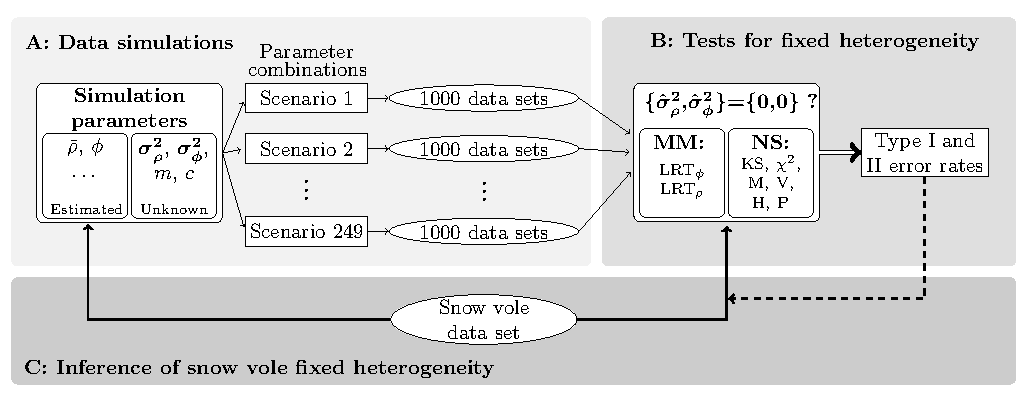
\includegraphics[width= \textwidth]{FiguresDynHet/Figure1}
		\caption{\footnotesize Illustration of the simulation and testing process. (A) Data simulation: The simulation model is parametrized using the life cycle and vital rates of a snow vole population, along with additional, unknown, parameters introducing fixed heterogeneity ($\sigma_{\phi}^2$ and $\sigma_{\rho}^2$) and dynamic heterogeneity ($m$ and $c$). Different combinations of these simulation parameters define 249 scenarios. For each scenario, 1000 data sets are simulated. (B) Tests for fixed heterogeneity: Each simulated data set is tested for the presence of fixed heterogeneity with both mixed models (\MM) using likelihood ratio tests (LRT) on survival ($\phi$) and reproduction ($\rho$), and neutral simulations (\NSM), using six different tests (see main text). Because $\sigma_{\phi}^2$ and $\sigma_{\rho}^2$ are known for each simulated data set, we can estimate the type I and type II error rates under each scenario. (C) Analysis of the snow vole data: Both \MM and \NSM are applied to the real snow vole data set, and the outcome is interpreted in the light of the estimated error rates of each test.}
	\label{figure:flow}
\end{figure}
%%%%%%%%%%%%%%%%%%%%%%%%%%%%%%%%%%%%%%%%%%%%%%%%%%%%%%%%%%%%%%%%%%%%%%%%%%%%%%%%%%%%%%%%%%%%%%%%%%%%
%%%%%%%%%%%%%%%%%%%%%%%%%%%%%%%%%%%%%%%%%%%%%%%%%%%%%%%%%%%%%%%%%%%%%%%%%%%%%%%%%%%%%%%%%%%%%%%%%%%%
%%%%%%%%%%%%%%%%%%%%%%%%%%%%%%%%%%%%%%%%%%%%%%%%%%%%%%%%%%%%%%%%%%%%%%%%%%%%%%%%%%%%%%%%%%%%%%%%%%%%
\section{Results}
Mean ARS had no effect on the error rates of any test, so we merged together the the scenarios differing only by mean ARS. Therefore, all error rates are estimated based on 3000 tests (1000 data sets per scenario, times three mean ARS values).

\subsection{Type I error rates}
In the absence of simulated individual fixed heterogeneity and non-random transition probabilities between successive stages, all tests have a low rate of null-hypothesis rejection (table \ref{table:t1error}). This means that any discrepancy between \NSM and \MM must come from a difference in type II rather than type I error rates.
\begin{table}[H]
\caption{Type I error of tests used in the \MM and \NSM approaches, when applied to data sets without underlying fixed heterogeneity and with fully random transition probabilities}
\begin{center}\scriptsize
\begin{tabular}{c c c c c c c c c c}
\toprule
& \multicolumn{2}{c}{Mixed models} & & \multicolumn{6}{c}{Neutral simulations}\\
\cmidrule{2-3} \cmidrule{5-10}%\cmidrule(r) would trim the line
& LRT$_\rho$ & LRT$_\phi$ & & KS & $\chi^2$ & H & P & M & V\\
\midrule
estimate & 0.042 			& 0.000 		& & 			0.000 & 0.021				& 0.018 			& 0.039 			& 0.000 		& 0.000\\
95\% CI & 0.039;0.054 &	0;0.001		& & 	0;0.001		& 0.016;0.027	& 0.014;0.023	& 0.033;0.047	& 0;0.001		&	0;0.001	\\
\bottomrule
\end{tabular}
\end{center}
{\scriptsize Note: Type I error rates are estimated as the proportion of simulated data sets, generated without fixed heterogeneity nor Markovian process, for which a test provides a $p$-value below 0.05. Hence, each proportion is estimated from 3,000 tests. The 95\% CI (confidence intervals) are Wilson score intervals. $\mathrm{LRT}_\rho$ and $\mathrm{LRT}_\phi$ refer to the Likelihood Ratio Tests of the variance associated with the individual random intercept in reproductive success and survival, respectively. KS refers to a Kolmogorov-Smirnov test, and $\chi^2$ to a $\chi^2$ test, both of which compare the Lifetime Reproductive Success (LRS) distribution in a focal data set to the distribution of LRS distributions obtained through neutral simulations (\NSM). The four other tests are based on the distribution of values obtained by \NSM compared to the value in the focal data set (mean (M) and variance (V) of the LRS distribution; and entropy (H) and persistence (P) of the transition matrix between successive annual reproductive successes.}
\label{table:t1error}
\end{table}

\subsection{Type II error rates}
\subsubsection{Simulations with explicit fixed heterogeneity}
\paragraph{Neutral simulations (\NSM)}
The Kolmogorov-Smirnov test comparing LRS distributions is significant for only one simulated data set (pertaining to the scenario \{$\sigma_{\rho}^2=1, \sigma_{\phi}^2=2, \bar{\rho}=50\}$) out of the 72,000 data sets with explicit fixed heterogeneity on the transformed scale. For the parameter range simulated, this test has thus effectively null power. Nevertheless, $p$-values decrease with increasing $\sigma_{\rho}^2$ and $\sigma_{\phi}^2$ (for \{$\sigma_{\rho}^2=0, \sigma_{\phi}^2=0, \bar{\rho}.\}$ $\overline{p\textrm{-value}}=0.998$, $\mathrm{SE}=0.001$; for \{$\sigma_{\rho}^2=2, \sigma_{\phi}^2=2, \bar{\rho}. $ \} $\overline{p\textrm{-value}}=0.776$, $\mathrm{SE}=0.032$), showing that the extremely low power is not the result of a complete calculation failure. Similar to the results of \cite{Plard2012}, the $\chi^2$ test is more powerful than the Kolmogorov-Smirnov test. Nevertheless, statistical power remains below 0.8 for moderately sized simulated variances, and its maximal value is 0.89 for the highest simulated variances (figure \ref{figure:VarIn}(A)).

Tests based on mean LRS are non-significant for all data sets and every scenario. The power of tests based on the variance in LRS increases with increasing $\sigma_{\phi}^2$, while the power peaks at intermediate values of simulated $\sigma_{\rho}^2$ and decreases again for higher $\sigma_{\rho}^2$ (figure \ref{figure:VarIn}(B)). The non-monotonic shape might be the result of the simultaneous increase in both the real observed-expected difference and the sampling variance: As the simulated variances go up, the LRS distribution becomes wider and flatter. Keeping the number of \NSM constant, this results in a less extensive sampling of the LRS distribution and a reduced power.

Tests based on the entropy of transition matrices display a pattern that is similar to that for $\chi^2$ tests, albeit with lower statistical power, this time peaking at 0.57 (figure \ref{figure:VarIn}(C)).
Tests based on the persistence of transition matrices have high statistical power ($\approx  0.8$) for $\sigma_{\rho}^2 \geq 1$, while increases in $\sigma_{\phi}^2$ result only in a slight increase in statistical power (figure \ref{figure:VarIn}(D)). While they reach higher statistical power than the $\chi^2$ tests, they have lower power than the $\chi^2$ at intermediate $\sigma_{\rho}^2$ values.

\paragraph{Mixed models (\MM)}
In contrast to \NSM, the power of the likelihood ratio test for ARS ($LRT_{\rho}$) is almost perfect for $\sigma_{\rho}^2 \geq 0.1$. Even though fixed heterogeneity in reproduction and survival are simulated independently, the power to detect fixed heterogeneity in reproduction is marginally influenced by the value of $\sigma_{\phi}^2$ (figure \ref{figure:VarIn}(E) and, more clearly, Appendix \ref{app:orsc} figure \ref{app:orsc}\ref{figure:VarOut}(E)). This is because a higher variance in latent survival probability increases the proportion of individuals that reach the maximal age, which provides more successive observations of reproduction and thereby increases the power to detect variance in reproductive quality. Overall, $\sigma_{\rho}^2$ is slightly underestimated ($\hat{\sigma_{\rho}^2} = 0.972 \sigma_{\rho}^2$; adjusted R$^2$=0.9997).

The $LRT_\phi$ is never significant, even for $\sigma_{\phi}^2=2$. Moreover the estimation of $\sigma_{\phi}^2$ is always close to zero (average of the median values 0.029) and does not increase with increasing $\sigma_{\phi}^2$ (slope and SE: $-0.0016 \pm 0.0006$). The failure of this model illustrates the intrinsic difficulty in estimating random effects for binary traits, especially when there are few repeated measurements per individual \parencite[e.g.][chapter 9]{Albert1984,Hosmer2013}, as is the case in our short-lived simulated animals.

\begin{figure}[H]
	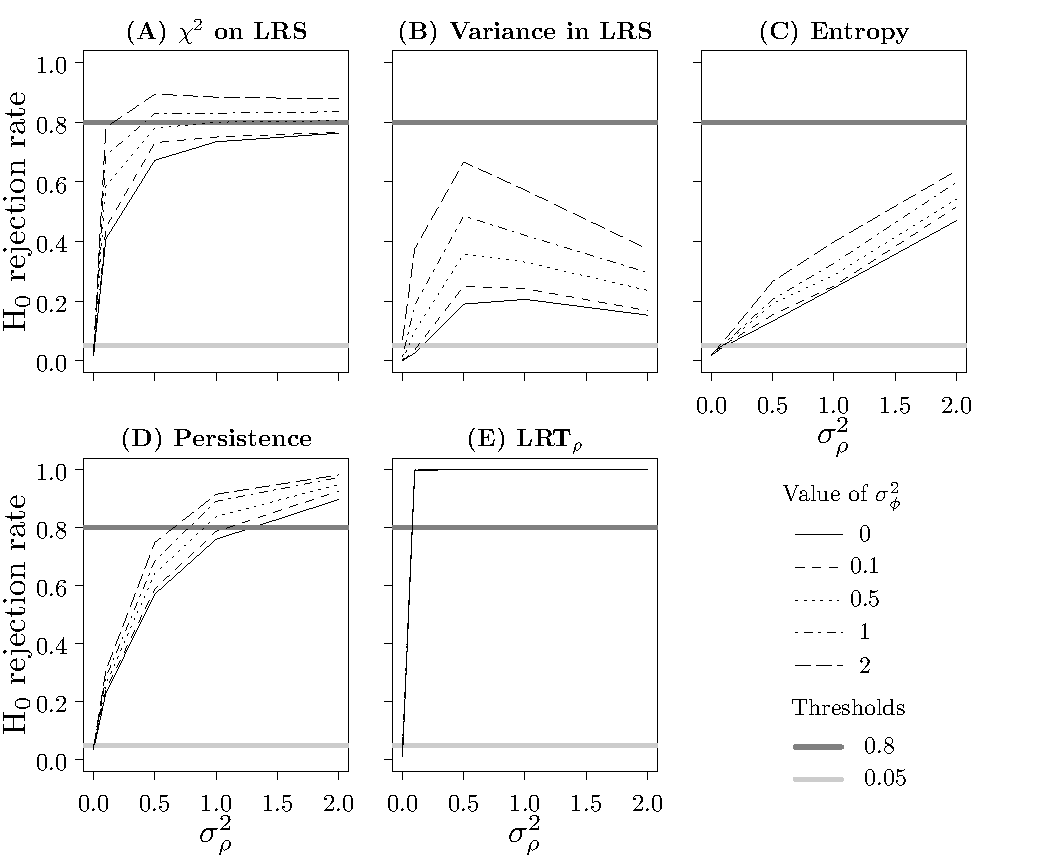
\includegraphics[width=\textwidth]{FiguresDynHet/Figure2}
		\caption{ \footnotesize Null-hypothesis rejection rates for various methods testing for the presence of fixed heterogeneity, as a function of the variance in reproductive propensity, $\sigma_{\rho}^2$, and survival propensity, $\sigma_{\phi}^2$, when these variances are introduced on the transformed scales. The methods are: (A) a $\chi^2$ test comparing the LRS distribution in a focal data set to the distribution of LRS distributions obtained through the neutral simulation approach (\NSM); tests based on proportion of values obtained by \NSM greater or equal to the value in the focal data set for (B) the variance in LRS, (C) the entropy of the transition matrix between successive annual reproductive success and (D) the persistence of this matrix; (E) a LRT for the significance of the individual random intercept in reproductive success. When $\sigma_{\rho}^2 = \sigma_{\phi}^2 = 0$, the null-hypothesis rejection rates are equal to the type I error rates, which is expected to be 0.05 (light gray line). When $\sigma_{\rho}^2 \neq 0$ or $\sigma_{\phi}^2 \neq 0$, the null-hypothesis rejection rates give (1-type II error rate), i.e. statistical power. The dark gray line indicates the 0.8 threshold. (A)-(D) are related to \NSM, (E) is related to \MM.}
	\label{figure:VarIn}
\end{figure} 	

\subsection{Simulations with a Markovian process}
Although data sets simulated using a Markovian process do not contain explicit fixed heterogeneity, both \MM and \NSM reject the null hypothesis of an absence of fixed heterogeneity in most of the cases (figure \ref{figure:Markov}).\\
The LRT$_\rho$, testing for fixed heterogeneity in ARS (based on \MM), rejects the null hypothesis with a high probability, except for the lowest values of $c$ and $m$ (figure \ref{figure:Markov}(E)). When $m > 0$, current ARS is influenced by past ARS, which in turn introduces variance in the propensity to reproduce. When $c > 0$, current survival probability is positively influenced by current ARS. As a consequence, successful reproducers live longer, resulting in more ARS values for these individuals, which improves the ability of the \MM to detect individual-level variance.
The LRT$_\phi$ is never significant for $c=0$, but rejects the null hypothesis at a high rate for $c \geq 0.5$, and this increases as $m$ increases (figure \ref{figure:Markov}(G)). This pattern was expected as $c$ controls the correlation between survival and reproduction, and indirectly makes the probability to survive in the current time step dependent on the probability to survive in the previous time step. Increasing values of $m$ further strengthen this correlation.

Both the Kolmogorov-Smirnov test on the LRS distribution, and the test based on mean LRS, are non-significant for any data set with Markovian process. Furthermore, the $\chi^2$ test rejects the null hypothesis with near certainty when $c>0$, and, when $c=0$, with probabilities going from low to moderate with increasing $m$ (figure \ref{figure:Markov}(A)). Given the absence of explicit fixed heterogeneity in these data, the $\chi^2$ test can therefore be considered to have very high type I error rates (but see the discussion).
The tests based on the variance in LRS, entropy and persistence follow a similar pattern of increasing probability of null-hypothesis rejection when $m$ and $c$ increase, but the test based on entropy does not reach a probability higher than 0.65, while the two other tests are close to 1 for the highest values of the parameters (figures \ref{figure:Markov}(B)-(D)). 

Based on these findings, it could be argued that both \MM and Plard's version of \NSM \parencite{Plard2012} have a very high type I error rate when the transitions between stages are structured. We examine this interpretation in more detail in the discussion. 
However, the rejection rate of the LRT$_\rho$ for fixed heterogeneity in ARS is drastically reduced by the inclusion of the past ARS ($\rho_{i,t-1}$) in the two mixed models that are being compared, i.e. with and without the individual random effect (compare figure \ref{figure:Markov}(E) and figure \ref{figure:Markov}(F)). The type I error rate is greater than the alpha threshold of 5\% only when both $m > 0.8$ and $c > 0$ (figure \ref{figure:Markov}(F)). Moreover, the estimates of the variance in reproductive propensity are reduced by the inclusion of $\rho_{i,t-1}$ in the models: over all the scenarios, the mean is $\hat{\sigma_{\rho}^2}=0.004$, SE=0.002, with a maximal estimate of 0.144, whereas without including $\rho_{i,t-1}$, the mean is 0.050, SE=0.008, and the maximum 0.459. The former estimate is closer to zero, i.e. the individual-level variance that is explicitly simulated.

\begin{figure}[H]
	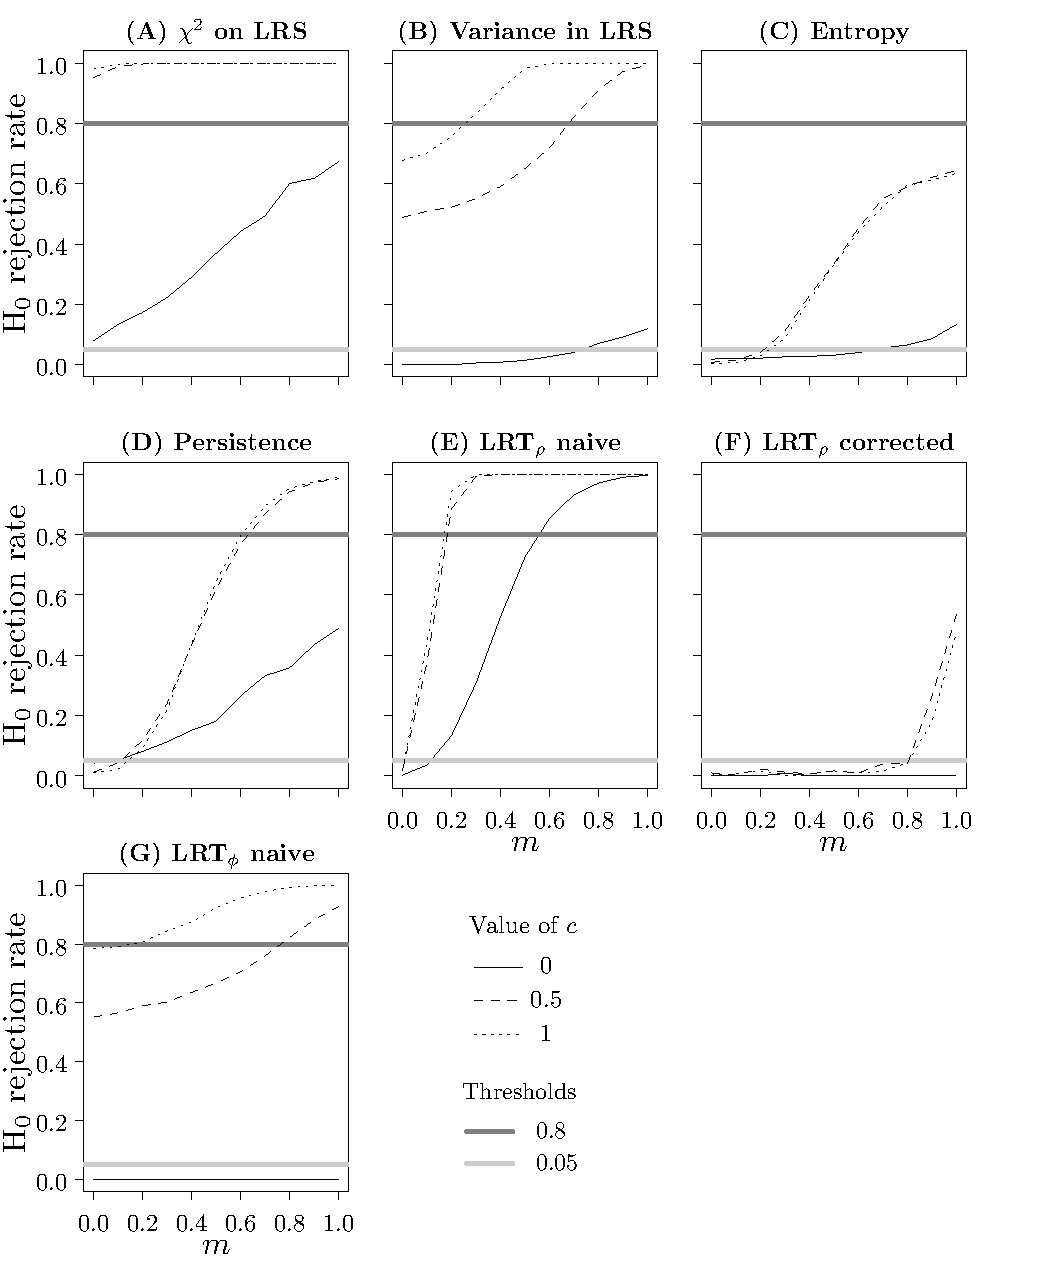
\includegraphics[width=\textwidth]{FiguresDynHet/Figure3}
	\caption{ \footnotesize Null-hypothesis rejection rates for various methods testing for the presence of fixed heterogeneity, when none is explicitly simulated, depending on the parameter $m$, controlling the structure of transitions between successive annual reproductive successes, and on the parameter $c$, controlling the dependency between survival probability and reproductive success (see the method section ``Simulations of a Markovian process'' for details). The methods are: (A) a $\chi^2$ test comparing the LRS distribution in a focal data set to the distribution of LRS distributions obtained through \NSM; tests based on proportion of values obtained by \NSM greater or equal to the value in the focal data set for (B) the variance in LRS, (C) the entropy of the transition matrix between successive annual reproductive success and (D) the persistence of this matrix; (E) a LRT for the significance of the individual random intercept in reproductive success, using models that do not account for a Markovian process, or (F) that do account for a Markovian process; (G) a LRT for the significance of the individual random intercept in survival. For survival we did not try to account for the Markovian process. Assuming that the simulated Markovian process cannot be related to fixed heterogeneity, the null-hypothesis rejection rates represent type I error rates for all values of the $c$ and the $m$ parameters. (A)-(D) are related to the \NSM framework. (E)-(G) are related to the \MM framework}
	\label{figure:Markov}
\end{figure}

%%%%%%%%%%%%%%%%%%%%%%%%%%%%%%%%%%%%%%%%%%%%%%%%%%%%%%%%%%%%%%%%%%%%%%%%%%%%%%%%%%%%%%%%%%%%%%%%%%%%
\subsection{Application to the snow vole data set}
\subsubsection{Neutral simulations (\NSM)}
For males, none of the six tests carried out within the \NSM framework are significant. Neither the LRS distribution, nor the transition matrix between successive values of ARS, are distinguishable from those generated using \NSM (table \ref{NS_table}).
For females, out of the six tests, two are significant: there is more persistence and more variance than expected under neutrality; and the test on mean LRS is close to being significant. However, the tests on the complete LRS distribution (Kolmogorov-Smirnov and $\chi^2$) are far from significant (table \ref{NS_table}). The latter is unsurprising as a graphical examination of the observed and the simulated neutral LRS distribution shows that the two distributions are almost indistinguishable (figure \ref{figure:LRS}).
According to the authors of the \NSM framework, the comparison of LRS distributions, either through a Kolmogorov-Smirnov test \parencite[in][]{Steiner2012} or a $\chi^2$ test \parencite[in][]{Plard2012}, is the gold standard when testing for the presence of fixed heterogeneity with \NSM (Steiner 2013, pers. comm. November 25th). Based on these \NSM results, there is thus no evidence for fixed heterogeneity in either of the sexes, although the results are more equivocal in females.

\begin{figure}[ht]
		%\subfigure[Females]
				{
					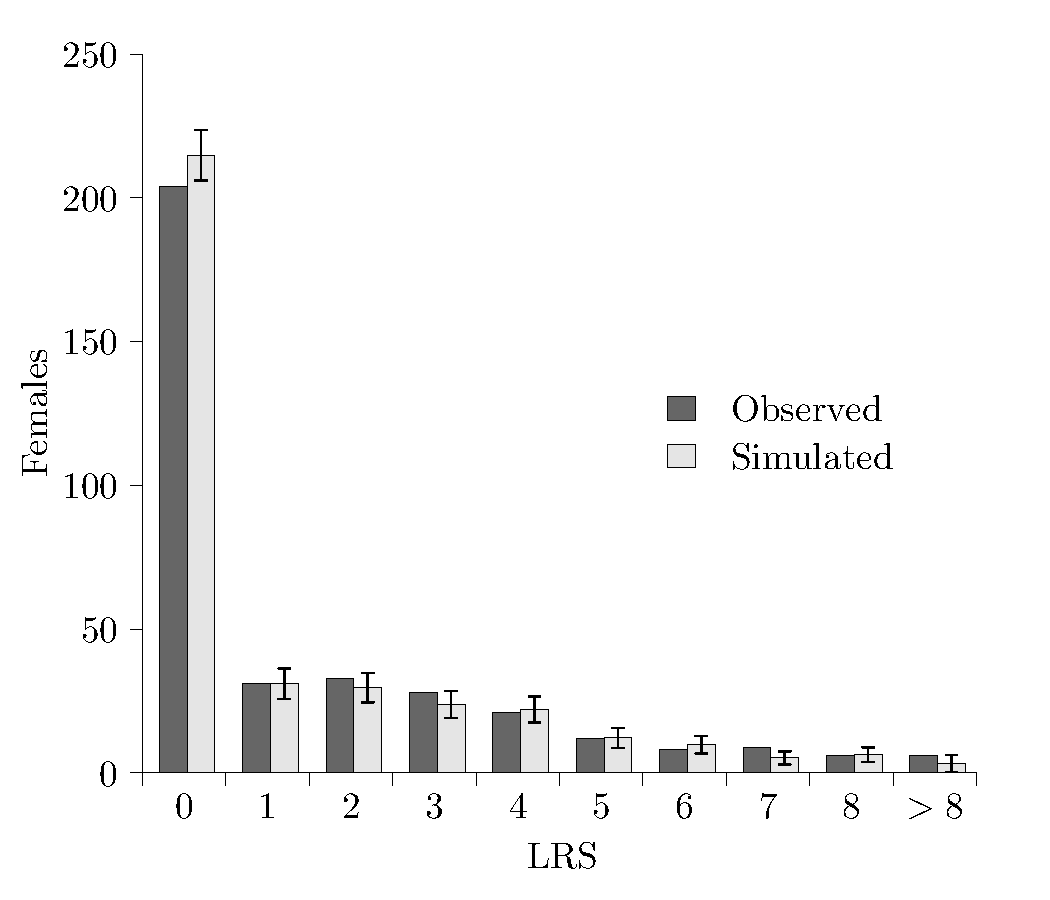
\includegraphics[width=0.5\textwidth]{FiguresDynHet/Figure4a}
					\label{figure:LRSF}
				}
		%\subfigure[Males]
				{
					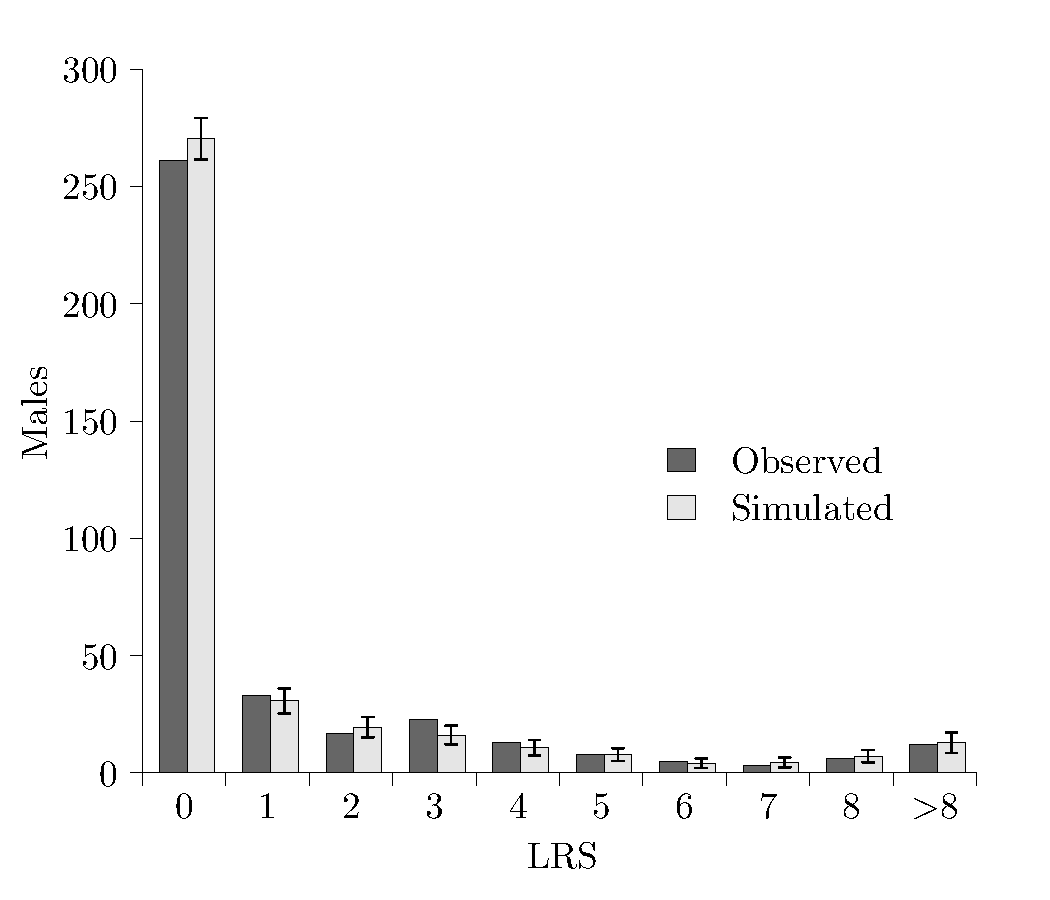
\includegraphics[width=0.5\textwidth]{FiguresDynHet/Figure4b}
					\label{figure:LRSM}
				}
\caption{ \footnotesize Distribution of lifetime reproductive success in the real snow vole data set, observed (dark bars) and simulated through 1000 neutral simulations (light bars with black error bars showing $\pm$ standard deviation), for \ref{figure:LRSF} females and \ref{figure:LRSM} males.WRONG}
				\label{figure:LRS}
\end{figure}

\begin{table}[ht]
\begin{center}
\caption{Outcomes of the various tests within the \NSM framework when applied to the real snow vole data set, for males and females separately} 
\label{NS_table}
\footnotesize
\begin{tabular}{cccccccccccc}
\toprule
\multirow{2}*{test} & \multicolumn{2}{c}{KS} & & \multicolumn{3}{c}{$\chi^2$} & & \multicolumn{1}{c}{H} & \multicolumn{1}{c}{P} & \multicolumn{1}{c}{V} & \multicolumn{1}{c}{M}\\
\cmidrule(r){2-3} \cmidrule(r){5-7} \cmidrule(r){9-12}
 & $D$ & $p$-value & & $\chi^2$ & df & $p$-value & & $p$-value & $p$-value &$p$-value &$p$-value \\
\midrule
Males  & 0.025 & 0.969 & & 8.33 & 15 & 0.909 & & 0.629 & 0.646 &0.395 & 0.378\\
Females  & 0.030 & 0.902 & & 5.50 & 8 & 0.70 & & 0.624 & \textbf{0.035} & \textbf{0.031} & 0.057 \\
\bottomrule
\end{tabular}
\end{center}
{\scriptsize Note: KS refers to the Kolmogorov-Smirnov test, and $\chi^2$ to the $\chi^2$ test, comparing the Lifetime Reproductive Success (LRS) distribution in a focal data set to the distribution of LRS distributions obtained through \NSM. The four other tests are based on the proportion of values obtained by \NSM greater than the value in the focal data set for the mean (M) and variance (V) of the LRS distribution, and for the entropy (H) and persistence (P) of the transition matrix between successive annual reproductive success. The $p$-values $ \leq $5\% are shown in bold.}
\label{table:NSCN}
\end{table}

\subsubsection*{Mixed models (\MM)} \label{sec:MMsv}
The GLMM for survival identifies significant between-years variance (5.622; 95\% CI $[1.133;13.158]$), but estimates a latent individual-level variance of 0 (95\% CI $[0;0.248]$) (see supplementary table \ref{Phi_table} for all the estimates of this model).

The GLMM for ARS estimates variances among individuals (0.371; 95\%CI $[0.151 ; 0.475]$) as well as among years (0.101; 95\%CI $[0.026 ; 0.452]$) that are different from zero, and LRTs for both variances are highly significant. The random effect accounting for overdispersion does not significantly differ from zero, although its bootstrapped confidence interval includes positive values (table \ref{Rho_table} for all the estimates of this model). When the individual random effect is not included, this overdispersion variance is highly significant, and the sum of squared Pearson residuals divided by the estimated residual degrees of freedom is approximately 2, while it falls to 1 with individual as a random effect. The estimation of residual degrees of freedom in GLMMs is a complex issue \parencite{Pinheiro2000}, but this approach seems to indicate that the overdispersion in the distribution is largely due to differences between individuals.

Excluding individuals reproducing for the first time, we fitted a GLMM that includes the previous reproductive success $\mathrm{ARS}_{t-1}$ and sex as fixed effects, and year as the only random effect. This model indicates a significant positive relationship between successive values of ARS (slope=0.0949; $\mathrm{SE}=0.0213$; $p$-value=$8 \times 10^{-06}$). Nevertheless, adding individual as a random effect greatly improved the fit of the model ($\Delta \mathrm{AIC}=87$; LRT: $p$-value $<10^{-16}$), providing evidence for the existence of significant individual-level variance ($\hat{\sigma_{id}^2}=0.341$, bootstrapped 95\% CI $[0.189;0.453]$). Including $\mathrm{ARS}_{t-1}$ had little effect on the estimate of $\hat{\sigma_{id}^2}$ (see table \ref{Rho_table}), but now $\mathrm{ARS}_{t-1}$ no longer reached significance (slope=0.0210; $\mathrm{SE}=0.0275$; $p$-value=0.445).

Finally, the latent correlation between the propensities to survive and to reproduce was estimated as 0.32 (95\% CI [-0.68;0.97]) and appears in the best model selected by DIC (see Appendix \ref{ap:cor}).

%%%%%%%%%%%%%%%%%%%%%%%%%%%%%%%%%%%%%%%%%%%%%%%%%%%%%%%%%%%%%%%%%%%%%%%%%%%%%%%%%%%%%%%%%%%%%%%%%%%%
%%%%%%%%%%%%%%%%%%%%%%%%%%%%%%%%%%%%%%%%%%%%%%%%%%%%%%%%%%%%%%%%%%%%%%%%%%%%%%%%%%%%%%%%%%%%%%%%%%%%
%%%%%%%%%%%%%%%%%%%%%%%%%%%%%%%%%%%%%%%%%%%%%%%%%%%%%%%%%%%%%%%%%%%%%%%%%%%%%%%%%%%%%%%%%%%%%%%%%%%%

%%%%%%%%%%%%%%%%%%%%%%%%%%%%%%%%%%%%%%%%%%%%%%%%%%%%%%%%%%%%%%%%%%%%%%%%%%%%%%%%%%%%%%%%%%%%%%%%%%%%
%%%%%%%%%%%%%%%%%%%%%%%%%%%%%%%%%%%%%%%%%%%%%%%%%%%%%%%%%%%%%%%%%%%%%%%%%%%%%%%%%%%%%%%%%%%%%%%%%%%%
%%%%%%%%%%%%%%%%%%%%%%%%%%%%%%%%%%%%%%%%%%%%%%%%%%%%%%%%%%%%%%%%%%%%%%%%%%%%%%%%%%%%%%%%%%%%%%%%%%%%
\section{Discussion}
\subsection{Overview}
Based on extensive simulations, we have shown that in the presence of fixed heterogeneity, \NSM have much less statistical power than \MM, even when the model simulating the data does not match the structure assumed by the \MM. In particular the Kolmogorov-Smirnov test, advocated in the earlier version of \NSM, has virtually no statistical power. In contrast, \MM have low type I error rates and are not misled by the presence of dynamic heterogeneity, which in all data sets is non-zero if it is measured as entropy \parencite{Tuljapurkar2009}. This finding directly contradicts the claim ``[\dots] that random effect models will always detect unobservable fixed effects'' \cite{Steiner2010}.
Second, in the absence of fixed heterogeneity, Markovian transitions between successive reproductive success and survival probabilities can induce high type I error rates, both in \MM and \NSM sensu \cite{Plard2012}. However, inclusion of previous reproductive success in the \MM for reproduction substantially reduces these errors.
Third, when applied to a real data set for a wild population of snow voles, \NSM only detect ambiguous deviations from neutrality and only for females. Moreover, the main tests of the framework, based on the total distribution of LRS, fail to reject the null hypothesis in both sexes. In striking contrast, \MM show strong evidence for individual latent variance in reproductive success, even when a Markovian process is accounted for. In addition, \MM give some indication of the presence of individual latent variance in survival, and of a positive correlation between survival and reproduction. However, the latter two parameters are estimated with substantial uncertainty.

\subsection{Use of simulations}
Testing methods on simulated data can be difficult because the specific simulation process used can differently match the assumptions and structures of the different methods. We tried to overcome this issue by using three different simulation models. 
Moreover, the rejection rates of \MM and \NSM observed in our simulations are similar to those observed when the methods are applied to real data. Indeed, in the present work we applied both methods to a snow vole data set and found that the \MM approach detected individual fixed heterogeneity, while the \NSM approach did not detect a significant deviation from the neutral expectation. This was also the case for the other data sets to which both methods were applied (\MM by \cite{Cam2013}; \NSM by \cite{Steiner2010}). On the whole we are aware of only a single case in which \NSM led to the rejection of neutrality  \parencite{Plard2012}, whereas \MM commonly find evidence for significant individual fixed heterogeneity, either by estimation of positive variance components, model selection \parencite{Cam2013} or posterior predictive checks \parencite{Chambert2014}. Although there is some possibility of publication bias, this pattern is consistent with our power analysis.

\subsection{Low power of Neutral Simulations}
The low power of \NSM probably stems from the fact that they aggregate data on vital rates, and that they do so twice: first over the lifetime of individuals, and then they aggregate individuals into population-level statistics. Thereby they first discard the repeatability of individuals, which has been shown to blur heritable differences among individuals \parencite{Vaupel1988}. Second, population-level statistics can be produced by an infinite number of different mixtures of individual types (for instance, a mean probability of 0.5 can be the result of a population consisting only of individuals with a latent probability of 0.5, or from a uniform distribution of individual probabilities between 0 and 1). Therefore, some patterns of among-individual differences are indistinguishable at the population level. Individual-level data are naturally better at identifying the causes of variation at that level \parencite{Cluttonbrock2010}, and the ability to use non-aggregated data, for instance longitudinal information on marked individuals, further increases this power \parencite{Brooks2013}. While a method such as Plard's \NSM could be valuable in the absence of such data, alternative methods making use of non-aggregated information, such as \MM, should be preferred whenever possible.

Importantly, within a strict null-hypothesis testing framework, the failure to reject a null hypothesis cannot be interpreted as a proof of the null hypothesis. The absence of significance in most implementations of the \NSM \parencite{Steiner2010,Orzack2011,Tuljapurkar2009,Plard2012} is therefore not informative with respect to the presence and the biological significance of fixed heterogeneity. The null-hypothesis testing framework can partially be relaxed by an a priori power analysis. Although comparisons of simulated data sets with and without heterogeneity were indeed presented in \cite{Steiner2012}, there fixed heterogeneity (assumed to be genetic) was modeled as two groups of homogeneous individuals, which except for clonal organisms is biologically unrealistic. In addition, the absence of significant differences between the data sets with and without fixed heterogeneity was not interpreted as a sign of a lack of statistical power, but as evidence that fixed heterogeneity has little effect on LRS distributions. 

\subsection{Effect of Markovian transitions}
When no fixed heterogeneity was explicitly simulated, both \MM and \NSM rejected the null hypothesis that fixed heterogeneity is absent. This was to be expected for \MM, given that Markovian transitions mimic individual-level variance, and \MM do not model population-level transition probabilities. It is more surprising that also \NSM had a high rate of false positives. However, we here used the ``full random model'' re-formulation of \NSM \parencite{Plard2012}, and not the ``full dynamic model'' \parencite{Tuljapurkar2009}. The latter simulates individual trajectories using a Markovian process, similar to the way data sets were simulated here, while the former simulates individual trajectories without taking into account the previous state.
Hence, ``full dynamic \NSM'' would not reject the null hypothesis, and one could consider this in this case to be correct. However, as latent individual quality will necessarily produce a pattern that is consistent with a Markovian process, this formulation does not allow for a complete separation of fixed and dynamic heterogeneity \parencite{Plard2012}.
Observing a Markovian process is therefore in itself not informative with respect to the mechanisms shaping life histories. Hence, although they have a low type I error rate, ``full dynamic \NSM'' always have low statistical power. 

We acknowledge that a Markovian process that is not due to fixed differences between individuals does mimic fixed heterogeneity, and thereby can bias estimates of between-individual variance based on full random \NSM and on \MM. Therefore, a naive \MM detects individual-level heterogeneity, irrespective of whether it is due to a population-level Markovian process or to individual-level differences. However, the type I error of \MM can be substantially reduced by including previous reproductive success in the model \parencite{Rotella2008, Cam2013}. Although this is not a universal solution that accounts for all confounding factors, it highlights the flexibility of the \MM framework, which allows for the incorporation of any factor that is perceived as potentially confounding based on knowledge of the study system. 

\subsection{Genetic variation as a source of fixed heterogeneity}
In cases where the evidence for the presence of fixed heterogeneity is equivocal, for instance because the effects of Markovian processes and individual-level fixed differences are confounded, the use of genetic information and quantitative genetic methods has the potential to tease apart latent genetic quality from other sources of performance persistence, including stochastic transitions.
Indeed, although other sources of variation may also generate fixed heterogeneity, the existence of significant additive genetic variation implies significant fixed heterogeneity, by definition determined at fertilization.
Interestingly, estimates of additive genetic variation for fitness components are often large, even in small populations \parencite[for reviews see][]{Mousseau1987, Postma2014}. As a matter of fact, when standardized by the mean (i.e. evolvability) rather than the variance (i.e. heritability), fitness components appear to have higher additive genetic variation than other types of traits \parencite{Hansen2011,Postma2014}. In addition to our findings, this provides further support for fixed heterogeneity being more common than suggested by \NSM.

\subsection{Interpretation of the snow vole results}
Because they are similar in structure, our simulated data sets can shed light on the results from the analysis of the real snow vole data set. For example, it is  unsurprising that the \MM fails to detect individual heterogeneity in snow vole survival probabilities. The LRT$_\phi$ has no statistical power for simulated data sets with simulated $\sigma_{\phi}^2 \leq 2$, while confidence and credibility intervals indicate that the possible values of $\sigma_{\phi}^2$ lay between 0 and 1 at most (supplementary tables \ref{Phi_table} and \ref{MCMCtable}).  
Unlike heterogeneity in individual survival probability, heterogeneity in individual reproductive success is easily detected and quantified by \MM applied to simulated data sets (figure \ref{figure:VarIn}(E)). Accordingly, the analysis of the real data set identifies an individual variance in the propensity to reproduce that is significantly different from zero, and is estimated to be more than three time larger than the variance among years. Finally, given the estimate of the variance $\sigma_{\rho}^2$, we can get an estimate of the statistical power of the other tests to detect fixed heterogeneity in the real snow vole data set: a significant test seems possible for the $\chi^2$ test (figure \ref{figure:VarIn}(A)), but quite unlikely for the test based on entropy (figure \ref{figure:VarIn}(C)).

A positive correlation between individual-level variation in reproduction and survival would provide further support for fixed heterogeneity. However, as mentioned above, the estimation of individual-level variance in survival is difficult because this is a binary trait, and because due to their short lifespan there are few observations per individual. Hence there is a lot of uncertainty in the estimation of this correlation parameter. Nevertheless, the most likely values are positive (Appendix \ref{ap:cor}).

\subsection{Fixed heterogeneity and the concept of fitness}
The debate surrounding the biological significance of fixed heterogeneity appears to stem at least partly from different concepts of fitness. On the one hand, proponents of the neutral theory of life histories consider fitness to be a property of a category of individuals, and consider variation in reproductive success among individuals to be mostly due to dynamic heterogeneity, rather than due to variation in latent individual properties \parencite{Steiner2012}. On the other hand, researchers in the field of evolutionary ecology often see fitness as a latent property of individuals \parencite{Cam2000}, that is, an expected value defined at the individual level that cannot be measured directly \parencite{Brandon1984,Price1996,Krimbas2004}. 
As the mean value of a group is also the expected value of an individual belonging to this group, the two views are not fundamentally different. In sexual organisms however, each individual is unique, which makes it difficult to assign it to a hypothetical group made of identical individuals. If stochastic variation underlies most of the realized reproductive success and there are no fitness differences between individuals, as adherents of the neutral theory of life histories advocate, then it is useless to define fitness at the individual level. However, if there exists significant fixed heterogeneity, individual performances carry some information about their latent properties, for example due to their genetic makeup. In the presence of fixed heterogeneity it therefore seems useful to use an individual-level definition of fitness, differing from both group-level fitness and realized reproductive success.

\section{Conclusions}
Using extensive simulations, we have demonstrated that \NSM are uninformative with respect to the biological significance of fixed heterogeneity.
Based on the work of \cite{Plard2012} and our power analysis, we conclude that the observation of a Markovian process in stage-transition probabilities does in itself not provide any biological insights. Within the \NSM framework, the full random model \parencite{Plard2012} should be preferred over the full dynamic model \parencite{Tuljapurkar2009}, and the $\chi^2$ test should be preferred over the Kolmogorov-Smirnov test. In addition, any use of \NSM should be complemented by an a priori power analysis, or otherwise be restricted to a strict null-hypothesis testing framework, where failure to reject the null hypothesis does not allow any conclusions regarding the null hypothesis being true, and/or the alternative hypothesis false. 
However, even when these improvements are included in the \NSM framework, we recommend that its use is restricted to data sets where individuals are not identified. 

Instead, we show that \MM are more powerful, but not more susceptible to type I error. Although \MM can be mislead by confounding factors, given a good knowledge of the biological system, it is possible to account for these confounding factors, in which case \MM have a very low type I error rate. 

Finally, the confrontation of our power analysis with the analysis of the real snow vole data set supports the presence of fixed heterogeneity in fitness components in this population. Further research is being carried out to identify what traits can be related to this latent heterogeneity, and how genetic and maternal effects shape these differences.

On the whole, this work supports the idea that fixed heterogeneity is more common than suggested by the studies based on \NSM. 

\section{Acknowledgments}
We thank Arpat Ozgul, Yannis Michalakis, Benjamin M. Bolker, Gordon A. Fox and an anonymous reviewer for helpful comments on this manuscript. Thanks to Ulrich K. Steiner for discussions on an earlier version of this work and for help with the implementation of neutral simulations. Thanks also to Lukas Keller, Josh Van Buskirk and Pirmin Nietlisbach for inspiring discussions on this topic. The snow vole monitoring was authorized by the \textit{Amt f\"{u}r Lebensmittelsicherheit und Tiergesundheit}, Chur, Switzerland. Funding was provided by the Swiss National Science Foundation project grant (\verb|31003A_141110|). 

%%%%%%%%%%%%%%%%%%%%%%%%%%%%%%%%%%%%%%%%%%%%%%%%%%%%%%%%%%%%%%%%%%%%%%%%%%%%%%%
%%%%%%%%%%%%%%%%%%%%%%%%%%%%%%%%%%%%%%%%%%%%%%%%%%%%%%%%%%%%%%%%%%%%%%%%%%%%%%%
\printbibliography[heading=subbibliography]

%%%%%%%%%%%%%%%%%%%%%%%%%%%%%%%%%%%%%%%%%%%%%%%%%%%%%%%%%%%%%%%%%%%%%%%%%%%%%%%
%%%%%%%%%%%%%%%%%%%%%%%%%%%%%%%%%%%%%%%%%%%%%%%%%%%%%%%%%%%%%%%%%%%%%%%%%%%%%%%
\newpage
\textbf{\LARGE{Supplementary information}}

\section{Checking the properties of the data sets}\label{ap:chpro}
The following Generalized Linear Models were fitted to the simulated data sets in order to test whether the data set properties matched the parameters used to generate them:

\begin{subequations}\label{eq:check}
\begin{align}
&\mathrm{logit}(\phi_{i,t})=\mu_{\phi}+\mathrm{Age}_{i,t}\label{eq:checkPA}\text{ ; using a binomial error structure}\\
&\mathrm{logit}(\phi_{i,t})=\mu_{\phi}+\rho_{i,t}\label{eq:checkPR}\text{ ; using a binomial error structure}\\
&\mathrm{log}(\rho_{i,t}) =\mu_{\rho}+ \rho_{i,t-1}\label{eq:checkRR}\text{ ; using a quasi-Poisson error structure}\\
&\mathrm{log}(\rho_{i,t}) =\mu_{\rho}+ \mathrm{Age}_{i,t}\label{eq:checkRA}\text{ ; using a quasi-Poisson error structure}
\end{align}
\end{subequations}

These were used to check that survival depended on age \eqref{eq:checkPA}, that survival depended on annual reproductive success only when that was required \eqref{eq:checkPR}, that ARS depended on previous reproductive attempts only when fixed heterogeneity for reproductive success or Markovian reproduction was simulated \eqref{eq:checkRR} and that ARS of adults was not age-dependent \eqref{eq:checkRA}. The simulated data had all the expected properties. Furthermore, we never found a significant association between reproduction and survival. This goes against the claim made in \cite{Steiner2010} that dynamic heterogeneity alone can generate a positive association between reproduction and survival.

Instead, we argue here that the findings on which they base their claim reflects their use of reproductive stage-specific survival in their \NSM, and reproduction and survival being positively correlated in the source data \parencite{Cam2002}. Hence, it is not the random transitions themselves that are responsible for the positive association, but the positively associated stage-specific probabilities of survival and reproduction. The origin of the latter remains unexplained, but is consistent with variation in latent fitness among individuals.

\section{Optimal number of neutral simulations per data set.}\label{ap:opnum}
The neutral simulation approach (\NSM) is computationally intensive: as the focal population consists of 10 cohorts of 100 individuals, performing 1000 neutral simulations (i.e. simulating 1000 hypothetical populations), requires 1,000,000 individual trajectories to be simulated for every simulated data set (and 75,000,000,000 individual trajectories for the complete study). To minimize computational time, we determined the number of neutral simulations per simulated data set beyond which statistical power did not change. Out of the six tests mentioned above, only $\chi^2$ tests on LRS distributions are sensitive to the number of neutral simulations; while $\chi^2$ tests based on 1000 neutral simulations differ from those based on 100 neutral simulations ($\Delta \mathrm{power}_{1000-100}$=-0.067, se=0.033), the tests based on 100,000 neutral simulations do not have more statistical power than those based on 1000 neutral simulations ($\Delta \mathrm{power}_{100,000-1000}$=-0.031, se=0.033), and the correlation of the statistical power across scenarios is high ($R^2=0.92$).
Accordingly, each simulated data set was analyzed using 1000 neutral simulations. Note that the fact that in this case statistical power plateaus already above 1000 neutral simulations is the result of the relatively short lifespan of the simulated animals, which allows for a quick exploration of all the possible individual trajectories. 

\section{Selection for latent quality}\label{ap:sel}

As outlined in the main document, we simulated fixed heterogeneity by attributing to each individual $i$ a fixed quality for annual reproductive success ($q_{\rho, i}$) and a fixed quality as survivor ($q_{\phi,i}$). These two kind of individual qualities are normally distributed, with mean zero and variance $\sigma_{\rho}^2$ and $\sigma_{\phi}^2$, respectively. The selection acting on, or due to, this variation in latent individual qualities for reproduction and for survival was measured as the individual-level covariance between the qualities and a proxy for fitness ($\omega$): relative lifetime reproductive success \parencite{Robertson1966}.

The selection coefficients increase with increasing variance in individual latent qualities, both for reproduction (figure \ref{ap:sel}\ref{figure:qua:rho}) and for survival (figure \ref{ap:sel}\ref{figure:qua:phi}). This confirms that the heterogeneity simulated is non-neutral. 

\begin{figure}[H]

%	\subfigure[Reproduction quality]
		{
			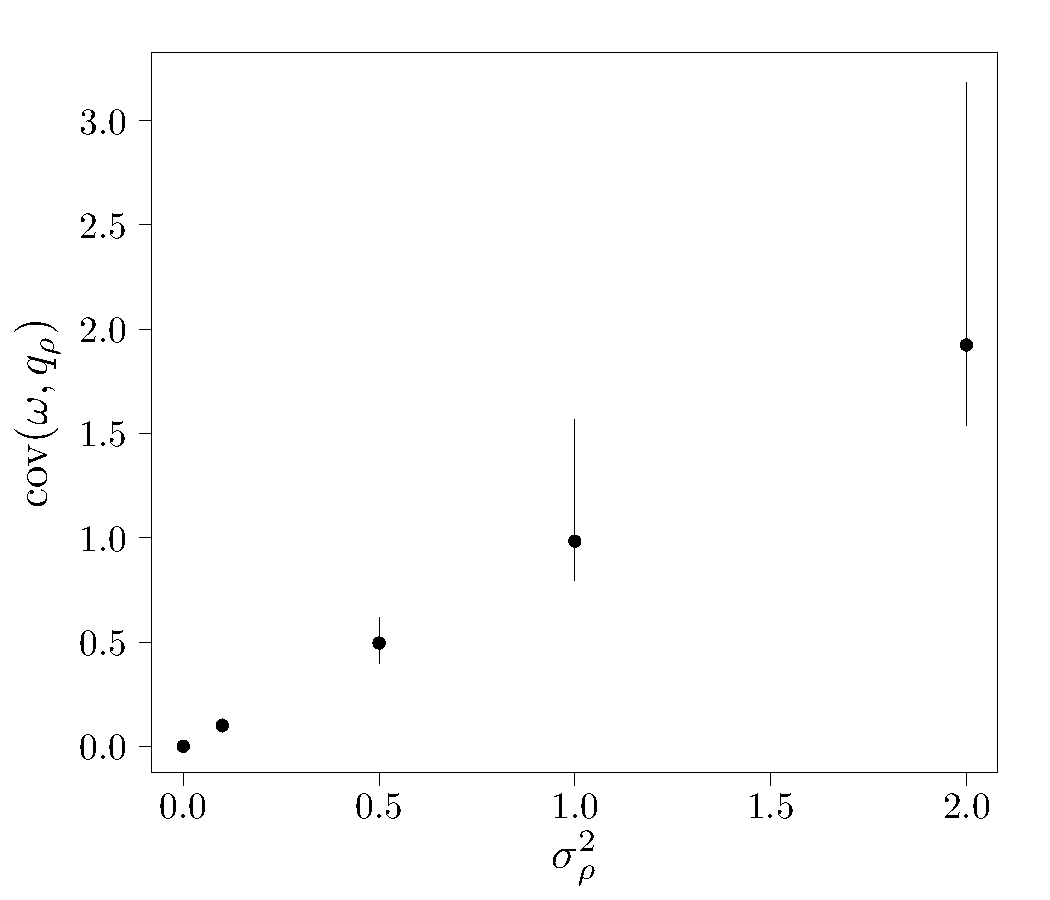
\includegraphics[width=0.5\textwidth]{FiguresDynHet/Figure5a}
			\label{figure:qua:rho}
		}
	%\subfigure[Survival quality]
		{
			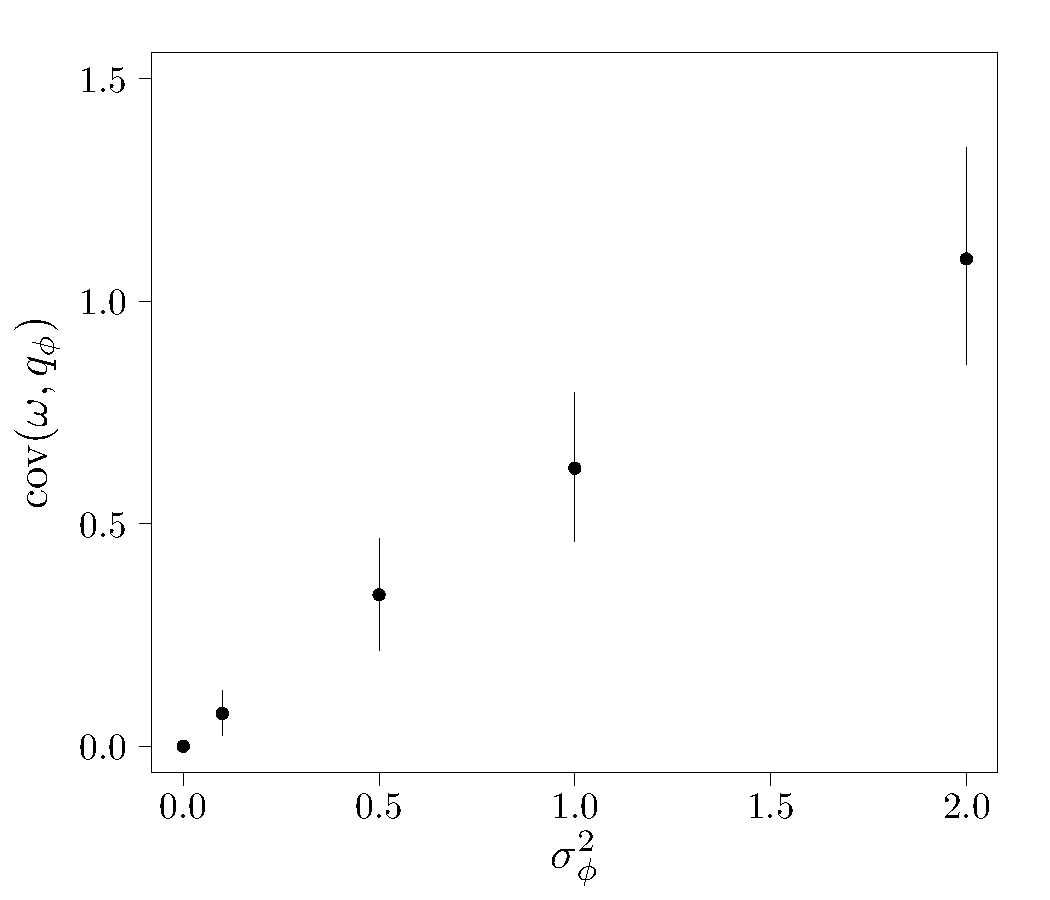
\includegraphics[width=0.5\textwidth]{FiguresDynHet/Figure5b}
			\label{figure:qua:phi}
		}
	\caption{ Appendix C \footnotesize Strength of selection on individual fixed qualities for survival and reproduction, as a function of the expected variance in these qualities. Strength of selection was measured as the individual-level covariance between the qualities and a proxy for fitness ($\omega$): relative lifetime reproductive success;  %\subref{figure:qua:rho} 
	for reproduction quality and %\subref{figure:qua:phi} 
	for survival quality. Vertical bars show the 95\% interval of the estimate distributions.}
	\label{figure:qua}
\end{figure}

\section{Simulating fixed heterogeneity on the original scale}\label{app:orsc}
It could be argued that the superior statistical power of the  $\mathrm{LRT}_{\rho}$ is the result of the simulation process used to introduce fixed heterogeneity has the same structure as the \MM estimating it. To address this, additional simulations were performed in which individual reproductive success and survival probability depended on their qualities on the original scale rather than on a transformed scale. Otherwise simulations were similar to those where fixed heterogeneity was introduced on the transformed scale. To this end, the reproductive success and survival of an individual $i$, at time $t$, are drawn from

\begin{subequations}\label{eq:varout}
\begin{align}
\rho_{i,t} &\sim \text{{\fontfamily{pzc}\selectfont P }}(\mu_{\rho}+q_{\rho,i})\\
\text{and } \phi_{i,t} &\sim \text{{\fontfamily{pzc}\selectfont B }}(\mu_{\phi}+\beta_{age}+q_{\phi,i}).
\end{align}
\end{subequations}


Although when the variance in quality for reproduction is included on the original, non-transformed, scale, mean reproductive success ($\overline{\mathrm{ARS}}$) has a dramatic negative influence on the power of the different tests, the hierarchy in the performance of the different tests does not change across the values of mean reproductive success. Therefore, we chose to present the results with pooled $\overline{\mathrm{ARS}}$ only (figure \ref{figure:VarOut})
Furthermore, it should be noted that although the $\sigma_{\rho}^2$ parameter values are the same in this section as in the previous one (0,0.1,0.5,1 and 2), they correspond to much smaller realized variances, as the variance is introduced on the original scale and not on a log-scale as previously. For correspondence between the variances on the two scales, see table \ref{table:Vlink}. 

\begin{table}[h]
\caption{Realized variance on the log scale as a function of variance introduced on the original scale ($\sigma_{\rho}^2$) and  mean reproductive success ($\overline{\rho}$)}
\begin{center}
\footnotesize
\begin{tabular}{c c c c c c}
\toprule
\multirow{2}{*}{$\overline{\mathrm{ARS}}$} &\multicolumn{5}{c}{$\sigma_{\rho}^2$ on original scale}\\
\cmidrule(r){2-6}
 & 0 & 0.1 & 0.5 & 1 & 2\\
\midrule
3 & 0 & 0.01143 & 0.06649 & 0.16947 & 0.39091 \\
10 & 0 & 0.00100 & 0.00506 & 0.01027 & 0.02108 \\
50 & 0 & 0.00004 & 0.00020 & 0.00040 & 0.00079 \\
\bottomrule
\end{tabular}
\end{center}
\label{table:Vlink}

{\scriptsize Note: Each realized variance was estimated from the variance of the log of 1,000,000 draws from a normal distribution of mean $\overline{\rho}$ and variance $\sigma_{\rho}^2$.}
\end{table}

\begin{figure}[H]
		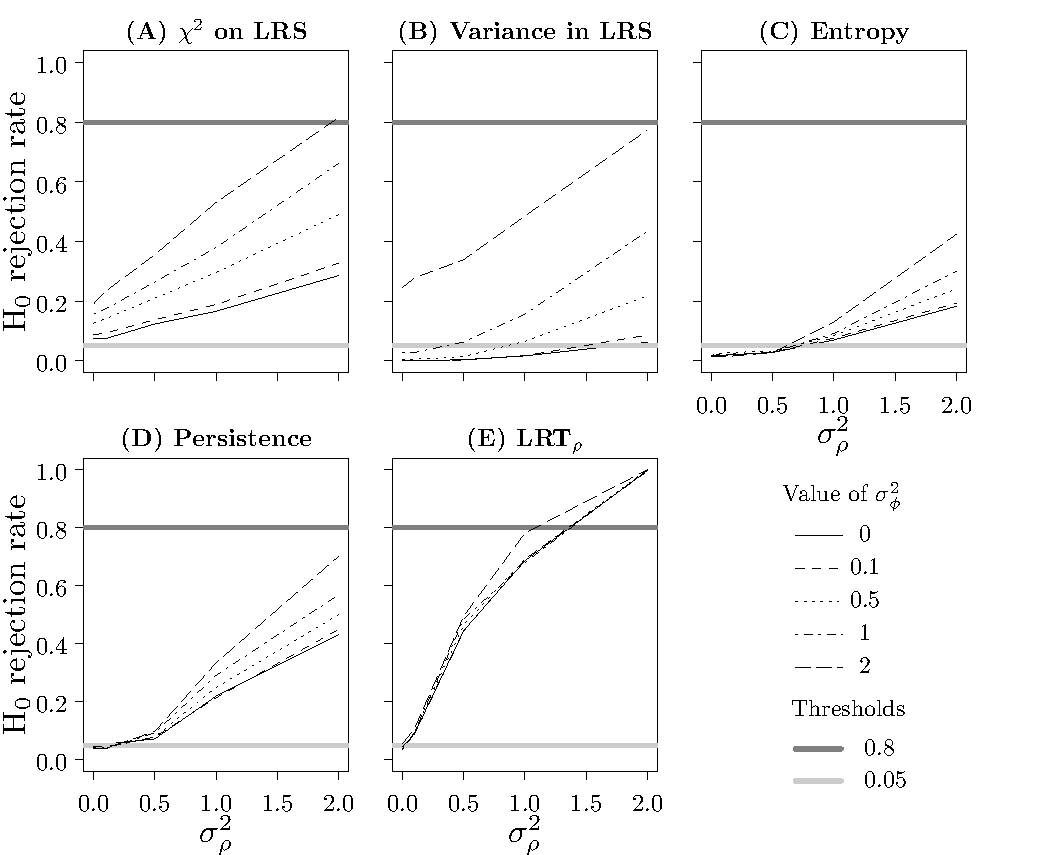
\includegraphics[width=\textwidth]{FiguresDynHet/Figure6}
	\caption{Appendix D \footnotesize Null-hypothesis rejection rates for various methods testing for the presence of fixed heterogeneity, depending on the variance in reproductive propensity, $\sigma_{\rho}^2$, and on the variance in survival propensity, $\sigma_{\phi}^2$, when these variances are introduced on the original scales. The methods are: (A) a $\chi^2$ test comparing the Lifetime Reproductive Success (LRS) distribution in a focal data set to the distribution of LRS distributions obtained through the neutral simulation approach (\NSM); tests based on proportion of values obtained by \NSM greater or equal to the value in the focal data set for (B) the variance in LRS, (C) the entropy of the transition matrix between successive annual reproductive success and (D) the persistence of this matrix; (E) a Likelihood Ratio Test for the significance of the individual random intercept in reproductive success. When $\sigma_{\rho}^2 = \sigma_{\phi}^2 = 0$, the null-hypothesis rejection rates are equal to the type I error rates, which is expected to be 0.05 (light gray line). When $\sigma_{\rho}^2 \neq 0$ or $\sigma_{\phi}^2 \neq 0$, the null-hypothesis rejection rates give (1-type II error rate), i.e. statistical power, which should be above 0.8 (dark gray line). (A)-(D) are related to \NSM, (E) is related to \MM.}	
	\label{figure:VarOut}
\end{figure}

\section{The snow vole population}\label{ap:snv}
\setcounter{table}{0}
\setcounter{equation}{0}
\setcounter{figure}{0}
A snow vole population, located in the central eastern Alps near Churwalden, Switzerland ($46^{\circ}$48' N, $9^{\circ}$34' E) at 2000m above sea level, has been monitored continuously since 2006. Analyses presented here are based on data collected until 2013. The study site consists of scree, which is the favourite habitat of the species, interspersed by patches of alpine meadows and surrounded by forest and larger meadows, which are not suitable habitats \parencite{Janeau1997}. Four trapping nights are necessary for sampling the complete area. Trapping throughout the whole study area took place two (in one year), three (in three years) or five times (in four years), between late May and mid-October. 

Unknown individuals were marked with a subcutaneous passive transponder (PIT, ISO transponder, Tierchip Dasmann, Tecklenburg) and an ear tissue sample was taken (maximum 2mm diameter, Thumb Type Punch, Harvard Apparatus) and stored in 90\% ethanol at $-20^{\circ}\mathrm{C}$. DNA extracted from the tissue samples was genotyped for 18 specific autosomal microsatellites developed for this population \parencite{Wandeler2008}, and the \textit{Sry} locus was genotyped in order to confirm the sex of all individuals. To identify cases of PIT loss as well as recaptures of juveniles initially too light for PIT injection, an identity analysis in CERVUS v.3.0 \parencite{Marshall1998} was carried out to detect resampled individuals.
Parentage was assigned to all juveniles and all first-time captured adults by simultaneously reconstructing parentage and sibship using the R package MasterBayes \parencite{Hadfield2006}. Analyses were performed for each year separately assuming polygamy for males and females and a uniform genotyping error rate of 0.5\% for all 18 loci. Parentage was assigned using a parental pool of all adults present in the examined year and the previous year. Because some rare first year individuals reproduce at the end of the season, as evidenced by the observation of pregnant and lactating first year individuals, the ``juveniles'' were also included in the parental pool of a second analysis excluding parent-offspring mating. Thereby eight additional parentage links could be identified. There were no inconsistencies between the reconstructed pedigree and the transmission of two sex-specific markers: a polymorphic Y-chromosome locus developed for this population \parencite{Wandeler2011} and a fragment of the mitochondrial DNA control region, amplified using vole specific primers \parencite{Haring2000}. This pedigree was used to measure annual and lifetime reproductive success.

Apparent year-to-year survival could be obtained without mark-recapture modeling as the recapture probability on a given year was virtually 1: no animal was not captured in a year but captured later, and no animal was ever found to be a parent of a juvenile in a year when it had not been captured. This is not surprising since mark-recapture modeling within years estimated a between-occasion recapture probability of 0.924 (SE 0.012) for adults and of 0.814 (SE 0.030) for juveniles.


\section{Univariate models of survival and reproduction in the snow vole population}\label{ap:Uni}

The following two tables (\ref{Phi_table} and \ref{Rho_table}) present all the estimates from the univariate models used to estimate the individual-level variance in survival and reproductive propensities for the snow vole population.
% latex table generated in R 3.1.2 by xtable 1.7-4 package
% Wed Nov 12 18:14:03 2014
\begin{table}[H]
\begin{center}
\caption{Estimates of coefficient of the mixed model for survival in the real snow vole data set}\label{Phi_table}
\footnotesize
\begin{tabular}{ccccc}
  \toprule
 & Estimate & SE & $p$-value & Bootstrap 95\% CI  \\ 
  \midrule
	Random effects:\\
$\sigma_{id}^2$ & 0.000 & - & 0.500 & [0;0.248] \\ 
  $\sigma_{year}^2$ & 5.622 & - & $<10^{-16}$ & [1.133;13.158] \\ 
	\\
   Fixed effects:\\
intercept & -1.754 & 0.830 & 0.035 & [-3.393;-0.111] \\ 
  age (Juvenile) & 1.841 & 0.230 & 0.000 & [1.369;2.411] \\ 
  sex (Male) & 0.306 & 0.295 & 0.300 & [-0.389;0.93] \\ 
  age:sex & -0.705 & 0.333 & 0.034 & [-1.449;0.091] \\ 
   \bottomrule
\end{tabular}
\end{center}
{\scriptsize Note: $\sigma_{id}^2$ and $\sigma_{year}^2$ refer to the variance between individuals and between years, respectively. All estimates are shown on the latent scale. The $p$-values for the significance of the two random effects are computed through a one-sided LRT. No standard errors (SEs) are provided for random effects. Instead, confidence intervals are computed using 1000 parametric bootstraps. The significance of the fixed effects is computed through the default Gaussian approximation provided by the package \texttt{lme4}.}
\end{table}

\begin{table}[H]
\caption{Estimates of coefficients of the mixed model for annual reproductive success in the real snow vole data set} 
\label{Rho_table}
\begin{center}
\footnotesize
\begin{tabular}{ccccc}
  \toprule
 & Estimate & SE & $p$-value & Bootstrap 95\% CI  \\ 
  \midrule
	Random effects:\\
$\sigma_{obs}^2$ & $3.3 \times 10^{-10}$ & - & 0.499 & [ 0 ; 0.194 ] \\ 
  $\sigma_{id}^2$ & 0.371 & - & $<10^{-16}$ & [ 0.151 ; 0.475 ] \\ 
  $\sigma_{year}^2$ & 0.101 & - & $<10^{-16}$ & [ 0.026 ; 0.452 ] \\ 
	\\
   Fixed effects:\\
intercept & 0.724 & 0.131 & 0.000 & [ -0.254 ; 0.266 ] \\ 
  age (Juvenile) & -5.703 & 0.369 & $<10^{-16}$ & [ -7.425 ; -5.125 ] \\ 
  sex (Male) & 0.046 & 0.101 & 0.645 & [ -0.118 ; 0.200 ] \\ 
	\bottomrule
\end{tabular}
\end{center}
{\scriptsize Note: $\sigma_{id}^2$ and $\sigma_{year}^2$ refers to the variance between individuals and between years, respectively. $\sigma_{obs}^2$ is a dummy random effect having one level per observation and used to account for potential over-dispersion in Poisson GLMMs. The $p$-value testing for the significance of these three random effects is computed through a one-sided likelihood ratio test. The significance of the fixed-effects is computed through the default normal approximation provided by the package lme4. Confidence intervals are computed using 1000 parametric bootstraps. The interaction between sex and age was not estimable by lme4: its inclusion produced convergence warnings and its SE was above $10^4$, without affecting other parameter estimates, and therefore it was removed from the model.}
\end{table}
\clearpage

%%%%%%%%%%%%%%%%%%%%%%%%%%%%%%%%%%%%%%%%%%%%
\section{Estimation of the latent correlation between survival and reproduction}\label{ap:cor}
Here we provide additional details on the bivariate models to test for the latent correlation between the propensity to reproduce and the propensity to survive. See main text for more details on the univariate analyses.

In univariate models for reproduction fitted using \verb+lme4+, neither the sex by age interaction, nor the dummy random effect controlling for overdispersion was significant. With \verb+MCMCglmm+, the non-significance was confirmed by bivariate models using the deviance information criterion (DIC) and Bayesian credibility intervals for these two parameters. Moreover, by default \verb+MCMCglmm+ takes into account any overdispersion in a distribution assumed to be Poisson. Therefore we did not include these two explanatory variables in the final model. Posterior predictive checks revealed that the bivariate model correctly predicted the number of zeros for ARS (observed 820, predicted 807 $\pm$ 23). Moreover, the year-level covariance between survival and reproduction was estimated close to zero, and fixing it to zero improved DIC, so it was fixed to zero in the final model. Finally, the package \verb+MCMCglmm+ always includes a residual variance component for binary variables, although this variance is not estimable. We fixed this residual variance to 1, as suggested in the package course notes ({\footnotesize\verb+http://www.cran.r-project.org/web/packages/MCMCglmm/vignettes/CourseNotes.pdf+}).
This model can be written as:

\begin{equation*}
	\begin{pmatrix}
	\rho_{i,t}\\
	\phi_{i,t}
		\end{pmatrix}
		\sim	
	\begin{pmatrix}
	f_{\rho}\\
	f_{\phi}
	\end{pmatrix}	
	+
	\begin{pmatrix}
	\sigma_{\rho (year)}^2 & 0\\
	0 & \sigma_{\phi (year)}^2
	\end{pmatrix}	
	+
	\begin{pmatrix}
	\sigma_{\rho (ind)}^2 & \sigma_{\rho \phi (ind)}\\
	\sigma_{\rho \phi (ind)} & \sigma_{\phi (ind)}^2
	\end{pmatrix}	
	+
	\begin{pmatrix}
	\sigma_{\rho (res)}^2 & \sigma_{\rho \phi (res)}\\
	\sigma_{\rho \phi (res)} & \sigma_{\phi (res)}^2
	\end{pmatrix}	
\end{equation*}
where $f_{\rho}$ and $f_{\phi}$ denote the fixed part of the model and both include an intercept, sex, age and their interaction. The $\sigma^2$ terms refer to variances and the $\sigma_{\rho \phi}$ terms refer to the covariances between ARS and survival, either at the level of years $_{(year)}$, of individuals $_{(ind)}$ or of the residuals $_{(res)}$.

The correlation between the individual propensity to survive and to reproduce was then calculated as $\sigma_{\rho \phi (ind)} /	\sigma_{\rho (ind)} \sigma_{\phi (ind)} $.
We used 1000 MCMC samples from 1,100,000 iterations with a thinning of 1000 and a burn-in of 100000. We used a non-informative parameter expanded prior. The residual variance of survival was fixed to 1, as this variance is not identifiable in binomial models.
We then refitted the same model while fixing $\sigma_{\rho \phi (ind)}$, $\sigma_{\rho (ind)}^2$ or $\sigma_{\phi (ind)}^2$ to zero, in order to compare the DIC of the two models. Although model selection on the variance-covariance random components is an active area of research \parencite[e.g.][chapter 6]{Burnham2002}, the use of DIC has been shown to be robust, at least under some conditions \parencite{Wilberg2008,Barnett2010}.
All models were checked by graphically assessing convergence and good mixing, and using Heidelberg stationarity tests. Moreover, thinning was sufficient to keep all auto-correlations between successive samples below 0.05. 

The Bayesian bivariate model identifies variance in the ability to reproduce, $\sigma_{\rho (id)}^2$. Although it is smaller than in the univariate model (table \ref{MCMCtable}), it was still different from zero, as 97\% of the posterior sample is above 0.01 and removing the random effect from the model substantially increases the DIC (table \ref{DICtable}).
Similar to the univariate model, the estimate of the variance in the ability to survive is small, with a large uncertainty. Including this effect in a model improves (i.e. decreases) DIC in one instance (model 4 versus model 5) but not in another instance (model 2 versus model 3), see table \ref{DICtable}. However, this effect appears in the best model. There is thus a large uncertainty in the estimation of variance in the ability to survive and mixed evidence for its existence.
Similarly, the correlation between the two individual random effects is estimated with a large credibility interval overlapping 0 (table \ref{MCMCtable}), and the inclusion of this parameter improves only marginally the DIC of the models (table \ref{DICtable}). Nevertheless, the mode of the posterior distribution is positive and the effect is present in the best model. Altogether, these results provide limited support for the biological significance of the latent correlation between survival and reproduction.

\begin{table}[ht]
\caption{Deviance information criterion (DIC) and difference to the best model ($\Delta$DIC), for five bivariate models of ARS and survival with different individual random effect structures}
\label{DICtable}
\begin{center}
\footnotesize
\begin{tabular}{cccccc}
	\toprule
	model & $\sigma_{\rho (ind)}^2$ & $\sigma_{\phi (ind)}^2$ & $\sigma_{\rho,\phi (ind)}$& DIC & $\Delta \mathrm{DIC}$ \\
	\midrule
	1 & Yes & Yes & Yes & 2554.587 & 0.000\\
	2 & Yes & Yes & No & 2556.793 & 2.206\\
	3 & Yes & No & No & 2556.100 & 1.513\\
	4 & No & Yes & No & 2560.945 & 6.358\\
	5 & No & No & No & 2564.187 & 9.600\\
	\bottomrule
	\end{tabular}
	\end{center}
{\scriptsize	Note: A ``Yes'' indicates that the parameter was included in the model, a ``No'', that it was not. The parameters are $\sigma_{\rho (ind)}^2$, the individual-level variance in ARS; $\sigma_{\phi (ind)}^2$ the individual-level variance in survival; $\sigma_{\rho,\phi (ind)}$ the individual-level covariance between reproduction and survival. Note that it is possible to include $\sigma_{\rho,\phi}$ only when both $\sigma_{\rho (ind)}^2$ and $\sigma_{\phi (ind)}^2$ are also included in the model.}
\end{table}
	
\begin{table}[ht]

\caption{Variance and correlation components for a bivariate model of survival and reproduction} 
\label{MCMCtable}
\begin{center}
\footnotesize
\begin{tabular}{ccccc}
  \toprule
 & Posterior mode & 95\% CI \\ 
  \midrule
$\sigma_{\rho (ind)}^2$ & 0.167 &$[1.4\times 10^{-4};0.342]$ \\ 
  $\sigma_{\phi (ind)}^2$ &$8.9\times 10^{-3}$&$[9.4 \times 10^{-7};1.048]$ \\ 
  $\sigma_{\rho \phi (ind)}$ & 0.322 &$[-0.682;0.974]$ \\ 
   \\
$\sigma_{\rho (year)}^2$ & 0.122&$[0.030;0.917]$ \\ 
  $\sigma_{\phi (year)}^2$ & 7.585 &$[2.074;73.123]$ \\ 
   \\
	$\sigma_{\rho (res)}^2$ & 0.230 &$[1.4\times 10^{-4};0.342]$ \\ 
  $\sigma_{\phi (res)}^2$ & 1 & fixed \\ 
  $\sigma_{\rho \phi (res)}$ & 0.180 &$[-0.313;0.576]$ \\ 
	\bottomrule
\end{tabular}
\end{center}
{\scriptsize Note: 95\% CI shows 95\% highest posterior density intervals.}
\end{table}
